% !TeX spellcheck = en_GB
%  LaTeX support: latex@mdpi.com 
%  In case you need support, please attach all files that are necessary for compiling as well as the log file, and specify the details of your LaTeX setup (which operating system and LaTeX version / tools you are using).

%=================================================================
\documentclass[energies,article,submit,moreauthors,pdftex]{Definitions/mdpi} 

% If you would like to post an early version of this manuscript as a preprint, you may use preprint as the journal and change 'submit' to 'accept'. The document class line would be, e.g., \documentclass[preprints,article,accept,moreauthors,pdftex]{mdpi}. This is especially recommended for submission to arXiv, where line numbers should be removed before posting. For preprints.org, the editorial staff will make this change immediately prior to posting.

%--------------------
% Class Options:
%--------------------
%----------
% journal
%----------
% Choose between the following MDPI journals:
% biologics, jmp, eng, jor, nursrep, biophysica, gastroent, jox, adolescents, hygiene, taxonomy, business, nanomanufacturing, geography, compoundsacoustics, actuators, addictions, admsci, aerospace, agriculture, agriengineering, agronomy, ai, algorithms, allergies, analytica, animals, antibiotics, antibodies, antioxidants, applmech, applnano, applsci, arts, asc, asi, atmosphere, atoms, automation, axioms, batteries, bdcc, behavsci , beverages, bioengineering, biology, biomedicines, biomedinformatics, biomimetics, biomolecules, biosensors, bloods, brainsci, breath, buildings, cancers, carbon , catalysts, cells, ceramics, challenges, chemengineering, chemistry, chemosensors, chemproc, children, civileng, cleantechnol, climate, clockssleep, cmd, coatings, colloids, computation, computers, condensedmatter, cosmetics, cryptography, crystals, cyber, dairy, data, dentistry, dermatopathology, designs, diabetology, diagnostics, digital, diseases, diversity, drones, earth, econometrics, ecologies, economies, education, ejbc, ejihpe, electricity, electrochem, electronicmat, electronics, endocrines, energies, engproc, entropy, environments, environsciproc, epidemiologia, epigenomes, est, fermentation, fibers, fire, fishes, fluids, foods, forecasting, forests, fractalfract, fuels, futureinternet, futurephys, galaxies, games, gardens, gases, gastrointestdisord, gels, genealogy, genes, geohazards, geosciences, geriatrics, hazardousmatters, healthcare, hearts, heritage, highthroughput, horticulturae, humanities, hydrogen, hydrology, ijerph, ijfs, ijgi, ijms, ijtpp, immuno, informatics, information, infrastructures, inorganics, insects, instruments, inventions, iot, j, jcdd, jce, jcm, jcp, jcs, jdb, jfb, jfmk, jimaging, jintelligence, jlpea, jmmp, jmse, jne, jnt, jof, joitmc, journalmedia, jpm, jrfm, jsan, land, languages, laws, life, literature, livers, logistics, lubricants, machines, magnetochemistry, make, marinedrugs, materials, materproc, mathematics, mca, medicina, medicines, medsci, membranes, metabolites, metals, microarrays, micromachines, microorganisms, minerals, modelling, molbank, molecules, mps, mti, nanomaterials, ncrna, ijns, neurosci, neuroglia, nitrogen, notspecified, nutrients, obesities, oceans, ohbm, osteology, optics, organics, particles, pathogens, pharmaceuticals, pharmaceutics, pharmacy, philosophies, photonics, physics, plants, plasma, pollutants, polymers, polysaccharides, preprints , proceedings, processes, prosthesis, proteomes, psych, psychiatryint, publications, quantumrep, quaternary, qubs, radiation, reactions, recycling, religions, remotesensing, reprodmed, reports, resources, risks, robotics, safety, sci, scipharm, sensors, separations, sexes, signals, sinusitis, skins, smartcities, sna, societies, socsci, soilsystems, solids, sports, standards, stats, surfaces, surgeries, suschem, sustainability, world, symmetry, systems, technologies, telecom, test, tourismhosp, toxics, toxins, transplantology, tropicalmed, universe, urbansci, uro, vaccines, vehicles, vetsci, vibration, viruses, vision, water, wem, wevj, women

%---------
% article
%---------
% The default type of manuscript is "article", but can be replaced by: 
% abstract, addendum, article, benchmark, book, bookreview, briefreport, casereport, changes, comment, commentary, communication, conceptpaper, conferenceproceedings, correction, conferencereport, expressionofconcern, extendedabstract, meetingreport, creative, datadescriptor, discussion, editorial, essay, erratum, hypothesis, interestingimages, letter, meetingreport, newbookreceived, obituary, opinion, projectreport, reply, retraction, review, perspective, protocol, shortnote, supfile, technicalnote, viewpoint
% supfile = supplementary materials

%----------
% submit
%----------
% The class option "submit" will be changed to "accept" by the Editorial Office when the paper is accepted. This will only make changes to the frontpage (e.g., the logo of the journal will get visible), the headings, and the copyright information. Also, line numbering will be removed. Journal info and pagination for accepted papers will also be assigned by the Editorial Office.

%------------------
% moreauthors
%------------------
% If there is only one author the class option oneauthor should be used. Otherwise use the class option moreauthors.

%---------
% pdftex
%---------
% The option pdftex is for use with pdfLaTeX. If eps figures are used, remove the option pdftex and use LaTeX and dvi2pdf.

%=================================================================
\firstpage{1} 
\makeatletter 
\setcounter{page}{\@firstpage} 
\makeatother
\pubvolume{xx}
\issuenum{1}
\articlenumber{5}
\pubyear{2020}
\copyrightyear{2020}
%\externaleditor{Academic Editor: name}
\history{Received: date; Accepted: date; Published: date}
%\updates{yes} % If there is an update available, un-comment this line

%% MDPI internal command: uncomment if new journal that already uses continuous page numbers 
%\continuouspages{yes}

%------------------------------------------------------------------
% The following line should be uncommented if the LaTeX file is uploaded to arXiv.org
%\pdfoutput=1

%=================================================================
% Add packages and commands here. The following packages are loaded in our class file: fontenc, inputenc, calc, indentfirst, fancyhdr, graphicx,epstopdf, lastpage, ifthen, lineno, float, amsmath, setspace, enumitem, mathpazo, booktabs, titlesec, etoolbox, tabto, xcolor, soul, multirow, microtype, tikz, totcount, amsthm, hyphenat, natbib, hyperref, footmisc, url, geometry, newfloat, caption

\usepackage{textcomp, gensymb}
\usepackage{color}
\usepackage[table]{xcolor}
\usepackage{epstopdf}
\usepackage{subfig}
\usepackage[T1]{fontenc}

\epstopdfsetup{outdir=./figures/}
\definecolor{gray090}{gray}{0.90}

%=================================================================
%% Please use the following mathematics environments: Theorem, Lemma, Corollary, Proposition, Characterization, Property, Problem, Example, ExamplesandDefinitions, Hypothesis, Remark, Definition, Notation, Assumption
%% For proofs, please use the proof environment (the amsthm package is loaded by the MDPI class).

%=================================================================
% Full title of the paper (Capitalized)
\Title{Building Suitable Datasets for Soft Computing and Machine Learning Techniques from Meteorological Data Integration: A Case Study for Predicting Significant Wave Height and Energy Flux}

% Author Orchid ID: enter ID or remove command
\newcommand{\orcidauthorA}{0000-0001-8849-6036} % Add \orcidA{} behind the author's name
\newcommand{\orcidauthorB}{0000-0001-9773-6783} % Add \orcidB{} behind the author's name
\newcommand{\orcidauthorC}{0000-0002-2657-776X} % Add \orcidC{} behind the author's name
\newcommand{\orcidauthorD}{0000-0003-4564-1816} % Add \orcidD{} behind the author's name

% Authors, for the paper (add full first names)
%\Author{Firstname Lastname $^{1,\dagger,\ddagger}$\orcidA{}, Firstname Lastname $^{1,\ddagger}$ and Firstname Lastname $^{2,}$*}
\Author{Antonio Manuel G\'omez-Orellana $^{1}$*, Juan Carlos Fern\'andez $^{1}$*\orcidA{}, Manuel Dorado-Moreno $^{1}$*\orcidB{}, Pedro Antonio Guti\'errez $^{1}$*\orcidC{} and C\'esar Herv\'as-Mart\'inez $^{1}$*\orcidD{}}


% Authors, for metadata in PDF
%\AuthorNames{Firstname Lastname, Firstname Lastname and Firstname Lastname}
\AuthorNames{Antonio Manuel G\'omez-Orellana, Juan Carlos Fern\'andez, Manuel Dorado-Moreno, Pedro Antonio Guti\'errez and C\'esar Herv\'as-Mart\'inez}


% Affiliations / Addresses (Add [1] after \address if there is only one affiliation.)
%\address{%
%$^{1}$ \quad Affiliation 1; e-mail@e-mail.com\\
%$^{2}$ \quad Affiliation 2; e-mail@e-mail.com}
\address{%
$^{1}$ \quad Department of Computer Science and Numerical Analysis, University of Cordoba, 14071, C\'ordoba, Spain.}

% Contact information of the corresponding author
%\corres{Correspondence: e-mail@e-mail.com; Tel.: (optional; include country code; if there are multiple corresponding authors, add author initials) +xx-xxxx-xxx-xxxx (F.L.)}
\corres{Correspondence: am.gomez@uco.es (A.M.G.-O); jfcaballero@uco.es (J.C.F.); manuel.dorado@uco.es (M.D.-M.); pagutierrez@uco.es (P.A.G.); chervas@uco.es (C.H.-M.) }

% Current address and/or shared authorship
%\firstnote{Current address: Affiliation 3} 
%\secondnote{These authors contributed equally to this work.}
% The commands \thirdnote{} till \eighthnote{} are available for further notes

%\simplesumm{} % Simple summary

%\conference{} % An extended version of a conference paper

% Abstract (Do not insert blank lines, i.e. \\) 
\abstract{Meteorological data are extensively used to perform environmental learning. Soft Computing (SC) and Machine Learning (ML) techniques represent a valuable support in many research areas, but require datasets containing information related to the topic under study. Such datasets are not always available in an appropriate format and its preparation and pre-processing implies a lot of time and effort by researchers. This paper presents a novel software tool with an user-friendly GUI to create datasets by means of management and data integration of meteorological observations from two data sources: the \textit{National Data Buoy Center} and the \textit{National Centers for Environmental Prediction and for Atmospheric Research Reanalysis Project}. Such datasets can be created using buoys and reanalysis data through customisable procedures, in terms of temporal resolution, predictive and objective variables, and can be used by SC and ML methodologies for prediction tasks (classification or regression). The objective is providing the research community with an automated and versatile system for the casuistry that entails well-formed and quality data integration, potentially leading to better prediction models. The software tool can be used as a supporting tool for coastal and ocean engineering applications, sustainable energy production or environmental modelling; as well as for decision making in the design and building of coastal protection structures, marine transport, ocean energy converters and well-planned running of offshore and coastal engineering activities. Finally, to illustrate the applicability of the proposed tool, a case study to classify waves depending on their significant height and to predict energy flux in the Gulf of Alaska is presented.}

% Keywords
\keyword{Environmental Prediction; Renewable Energy Resource Evaluation; Meteorological Data; Reanalysis Data; Marine Energy; Soft Computing}  % List three to ten pertinent keywords specific to the article, yet reasonably common within the subject discipline.

% The fields PACS, MSC, and JEL may be left empty or commented out if not applicable
%\PACS{J0101}
%\MSC{}
%\JEL{}

%%%%%%%%%%%%%%%%%%%%%%%%%%%%%%%%%%%%%%%%%%
% Only for the journal Diversity
%\LSID{\url{http://}}

%%%%%%%%%%%%%%%%%%%%%%%%%%%%%%%%%%%%%%%%%%
% Only for the journal Applied Sciences:
%\featuredapplication{Authors are encouraged to provide a concise description of the specific application or a potential application of the work. This section is not mandatory.}
%%%%%%%%%%%%%%%%%%%%%%%%%%%%%%%%%%%%%%%%%%

%%%%%%%%%%%%%%%%%%%%%%%%%%%%%%%%%%%%%%%%%%
% Only for the journal Data:
%\dataset{DOI number or link to the deposited data set in cases where the data set is published or set to be published separately. If the data set is submitted and will be published as a supplement to this paper in the journal Data, this field will be filled by the editors of the journal. In this case, please make sure to submit the data set as a supplement when entering your manuscript into our manuscript editorial system.}

%\datasetlicense{license under which the data set is made available (CC0, CC-BY, CC-BY-SA, CC-BY-NC, etc.)}

%%%%%%%%%%%%%%%%%%%%%%%%%%%%%%%%%%%%%%%%%%
% Only for the journal Toxins
%\keycontribution{The breakthroughs or highlights of the manuscript. Authors can write one or two sentences to describe the most important part of the paper.}

%\setcounter{secnumdepth}{4}
%%%%%%%%%%%%%%%%%%%%%%%%%%%%%%%%%%%%%%%%%%
\begin{document}
%%%%%%%%%%%%%%%%%%%%%%%%%%%%%%%%%%%%%%%%%%

%%%%%%%%%%%%%%%%%%%%%%%%%%%%%%%%%%%%%%%%%%
%\setcounter{section}{-1} %% Remove this when starting to work on the template.

	\section{Introduction}
		
		A better understanding of the environment is of vital importance for science, contributing not only to more efficient exploitation of natural resources but also to the development of new strategies aimed at its protection. In that sense, meteorological observations provide an essential and valuable source of information which is widely used by researchers to address environmental learning, comprehension, prediction and conservation in numerous oceanic and atmospheric studies of a wide variety of areas (e.g. energy, climate change, agriculture, etc.). Some specific examples of the diversity of fields in which meteorological data can be used in are, among others: global solar radiation estimation \cite{SHAHRUKHANIS2019179}, directional analysis of sea storms \cite{LAFACE201545}, estimation of hybrid energy systems taking into account economic and environmental objectives\cite{Kumar2020}, wind power ramp events prediction \cite{DORADOMORENO2017428}, sea surface temperature prediction \cite{He2020}, study of the responses exhibited by plankton to fluid motions \cite{FUCHS2016109}, trends in solar radiation \cite{SILVA20101852} or simulation of extreme near shore sea conditions \cite{GOULDBY201415}. All these studies require a prior data collection and its adaptation to a specific format that allows the interpretation of them.
		
		Once quality and well-formed data are obtained, these can be used to extract information and build prediction models that explain the behavior of a certain problem. The choice of the appropriate model, either in engineering problems or in any other problem, is also an important factor in addition to data \cite{Alizadeh2019, Alizadeh2020}. \textcolor{blue}{In this sense, public and research organisms are increasingly promoting the use of open and robust datasets to boost policies coherent with the environmental exploitation, protection and conservation, as well as modelling tools available to the scientific community and decision-makers \cite{Manfren2020}}. Although Soft Computing (SC) and Machine Learning (ML) techniques have the ability to handle uncertainty in data and are extensively used for modelling purposes, the real challenge in modelling studies is due to the inadequacy of data, since the adequacy of the models depend mainly on the the quality of the information used, so that if a researcher does not have quality data there will be no quality models.
		
		Continuing with this line, special purpose software is usually developed to help researchers to advance in their studies related to energy and environmental modelling, becoming a great support for decision-making in the exploitation and protection of the environment. In \cite{Neeraj2020}, a software package in R called ``ForecastTB'' is developed for comparing the performance of distinct prediction methods, presenting the software as a stepping stone in ML automation modelling.
		In \cite{LO2015293}, an integrated simulation tool to optimise the design of bifacial solar panel with reflectors is presented. This tool can also be applied to study the efficiency of the solar cells. A framework for integrating information from offshore wind farms is implemented in \cite{NGUYEN2013150} in order to ease data interchange and enhance operation and maintenance practices. 
		In \cite{Roberta2020}, a new software tool named ``Storage LCA Tool`` is presented for comparing PCM - phase change materials- storage systems with conventional systems that do not involve energy storage, being beneficial for supporting decision-making on energy concepts for buildings.
		A risk assessment tool to improve safety standards and emergency management in onshore wind farms, is presented in \cite{ASTIASOGARCIA201648}. Raabe et al. \cite{RAABE2010213} developed two software tools, \textit{Model of Equilibrium of Bay Beaches} (MEPBAY) and \textit{Coastal Modelling System} (SMC), for supporting distinct operational levels of headland-bay beach in coastal engineering projects, and Motahhir et al. \cite{MOTAHHIR20199} developed an open hardware/software test bench for solar tracker.
		
		Marine energy prediction is currently a hot topic where meteorological data is used in. Marine Renewable Energy (MRE) is one of the most important renewable and sustainable energy sources available in our environment \cite{en12050787}, and it includes ocean thermal energy, marine tidal current energy and wave energy, among others. Its benefits and great potential \cite{ZEYRINGER20181281} make it one of the most relevant natural resources, playing a crucial role not only in the reduction of the emission of greenhouse gases but also in all other aspects involved in the difficult challenge of the transition to a low carbon footprint society \cite{en12091657, BREDE201344, Alizadeh2020a}. Wave energy exhibits a more stable power supply than wind energy and even solar energy. In recent years \textit{Wave Energy Converters} (WECs) \cite{FALCAO2010899} have been developed and widely installed, \textcolor{blue}{even arranged in array form \cite{Amini2020}}, to transform this wave energy into electricity, which can be injected into the electric network or supplied to existing offshore oil and gas platforms \cite{OLIVEIRAPINTO2019556} or seawater desalination plants \cite{FERNANDEZPRIETO2019546}, among others. WECs are mechanical devices that convert kinetic energy into electrical energy through either the vertical oscillation or the linear motion of waves. Nevertheless, waves are difficult to be characterised due to their stochastic nature, because of the influence of a large number of environmental factors that exert on them \cite{ochi1998}. As a consequence of this complexity, many aspects of WEC design, deployment and operation \cite{CROWLEY2018159, Abdelkhalik2016, 6898109} need a proper prediction of waves \cite{en11010011, Kaloop2020}, in order to maximise the wave energy extraction \cite{en80910370}. For this purpose WECs use wave \textit{flux of energy} ($F_e$) which can be calculated from the two most relevant wave parameters related to this aspect: \textit{significant wave height} ($H_s$) and \textit{wave energy period} ($T_e$).
		
		Currently, and as a support to traditional study procedures, SC and ML techniques \cite{Sang-Yong2014,Bishop:2006:PRM:1162264} are being widely used in numerous research fields related to classification, regression and optimisation tasks, obtaining significant improvements in the performance of the results, either in engineering \cite{Alizadeh2020}, energy or environmental problems \cite{Fi-John2019,Mosavi2019,GUO201816}. SC and ML methodologies can be used not only by experienced computer scientists but also by other researchers. For example, the well-known \textit{Waikato Environment for Knowledge Analysis} (WEKA) \cite{WEKA} software tool provides researchers with a wide collection of ML  algorithms. ML techniques have been already applied to tackle wave characterisation, accurately estimating $H_{s}$ and $T_{e}$ parameters \cite{DURANROSAL2017268, KUMAR2017605}, given that robustness of ML methods can tackle the previously explained difficulties in wave energy prediction. In \cite{Ali2020}, a reliable ML model based on multiple linear regression and covariant-weighted least square estimation for $H_s$ modelling is presented in order to predict significant wave height 30 minutes in advance. In \cite{Cornejo-Bueno2016}, an  approach for feature selection problems is developed and applied for $H_s$ and $F_e$ prediction in oceanic buoys, obtaining very good results. In \cite{Emmanouil2020}, a Bayesian Network system provides a helpful tool to support decision-making process of installation and maintenance operations in offshore wind farms using predictions of $H_s$, among others. In \cite{Shamshirband2020}, several ML methods are implemented and compared for the prediction of $H_s$ in the Persian Gulf, the extreme learning machine (ELM) providing the best results. The problem is that, in order to apply ML and SC techniques, it is essential to obtain datasets with relevant information about the issue under study, used to infer knowledge. Usually, these datasets are not publicly available in a friendly format, and their generation is the first step needed.
		
		The information to create these datasets related with MRE can be obtained from meteorological observations, but such information may be available in a inappropriate format and even contain missing values or measurements. Consequently, it is usually required to perform pre-processing tasks for improving the quality of the data, such as the replacement of missing values, outlier detection or data normalisation, among others. Furthermore, if more than one source of information is used to achieve a better characterisation of the problem under study \cite{JOHANSSON2015143, FERNANDEZ201544, Adams2010}, then a data integration process, denominated as the matching process in this document, has to be carried out by researchers to manually create the datasets with the needed information. Given that such process is of great relevance and has an extensive casuistry, the present work has been specially focused on it. Moreover, depending on the subject and the SC and ML technique to be applied, or even if the researcher considers other factors in order to enhance the performance obtained or have more in-depth conclusions, the datasets would have to be updated afterwards. In summary, many important details and different intermediate steps have to be considered when creating suitable datasets, specially when data integration is required, resulting in an extremely tedious task.
		
		The main purpose of this paper is to present a new open source tool for the creation of datasets integrated by meteorological variables from two sources of information. Given that the tool provides an user-friendly graphical interface, no knowledge in programming languages is needed. It also prevents researchers from performing the mentioned tedious work and greatly simplify all the steps involved in it, avoiding possible errors in the intermediate steps, at least as a preliminary study in certain areas where some kind of environmental prediction is needed. The meteorological data used by the tool come from two well-known sources of information: the \textit{National Oceanic and Atmospheric Administration} (NOAA) \textit{National Data Buoy Center} (NDBC) \cite{NOAA} and the \textit{National Centers for Environmental Prediction} (NCEP)/\textit{National Center for Atmospheric Research} (NCAR) \textit{Reanalysis Project} (NNRP or R1) \cite{Kalnay1996, Kistler2001}. The open source software tool presented in this work is named SPAMDA (Software for Pre-processing and Analysis of Meteorological DAta to build datasets). As SPAMDA performs all this data processing, it reduces the time involving these tasks and allows researchers focus on the study of the meteorological aspects of the observations. The datasets obtained are ready to be used as input for SC and ML techniques in prediction tasks (classification or regression), although researchers can use them for other purposes. These datasets contain one or more meteorological variables as inputs and one variable as target (variable to be predicted). The format of the generated datasets will be \textit{Attribute-Relation File Format} (ARFF) \cite{WEKA_ARFF}, which is the one used by WEKA. Besides, the datasets can also be generated in \textit{Comma-Separated Values} (CSV) format, enabling researchers to use others tools.
		
		In order to address the problem previously discussed, meteorological data integration from NDBC and NNRP and the casuistry that it entails, SPAMDA offers to researchers novelties and functionalities that will be detailed in Section \ref{sec:SPAMDA}, although some of them are briefly summarised below:

		\begin{itemize}
			\item The generation of datasets becomes a very easy and customisable task by means of the selection of different input parameters, such as predictive and objective variables, classification and regression, output discretisation (useful for ordinal regression) or prediction horizon, among others.
			
			\item The created datasets can be easily used by SC and ML tools. 
			
			\item It makes the researcher focus on environmental modelling, without having to worry about the development of scripts or mechanical tasks, avoiding laborious pre-processing procedures, that imply a great deal of time and endeavour in early stages of the research.
			
			\item It avoids possible researcher errors in the intermediate steps of the process, such as geographical coordinates conversion, missing values handling (dates or measurements not recorded) or different temporal resolution of the data collected, among others.
			
			\item It provides information about the quality and quantity of the data. SPAMDA allows preliminary studies of missing values (dates or measurements not recorded) in buoys managed by NDBC, so that the researcher can have an idea of the quality of the data recorded by the buoys and about their suitability for the intended purpose. In any case, SPAMDA allows data integration taking into account such missing values when needed by the user.
			
			\item Estimation of the amount of energy flux that can be produced at different prediction horizons: short-term, mid-term or long-term. Although this work does not focus on models performance, it should be taken into account that models tend to generalise worse with greater prediction horizons.
						
			\item It manages the extensive casuistry of data integration which can lead to incomplete datasets, described in Appendix \ref{app:AppendixA}.
			
			\item Possibility of selecting one or more reanalysis nodes near the localisation under study, which could provide a better description of the problem to achieve more accurate models.
			
			\item Although pre-processing is not the main objective of SPAMDA, the tool also provides some basic pre-processing filters on buoys measurements, such as normalisation and missing data recovery.
			
			\item It facilitates data management and well-organised storage of the datasets. Environmental studies in different geographical locations can be carried out by merely introducing and using other collected data.
			
			\item SPAMDA is distributed as open source tool, its modular design allows the implementation of new modules for managing meteorological data from others sources, benefiting future renewable energy and environmental research.
			
			\item It includes a user-friendly GUI, facilitating and greatly simplifying data management, and it is integrated with the Explorer environment of WEKA.
			
			\item It is multi-platform, and it can be used on any computer with Java regardless of the operating system.
		\end{itemize}
		
		Therefore, the functionalities and characteristics that SPAMDA offers make it a supporting tool for researchers, which could be used in applications related to coastal and ocean engineering, and also in marine energy prediction. In \cite{Kumar2020}, the estimation of energy supply sources in hybrid energy systems is based on the amount of energy that can be obtained by a marine energy system within a prediction horizon. Regulation of WECs to avoid malfunction or breakage, depending on the significant wave height and/or energy flux expected, as well as the possibility of reconfiguring them in order to maximise the wave energy extraction, is studied in \cite{CROWLEY2018159, Abdelkhalik2016}. The prediction of the energy that could be obtained from a certain maritime location is considered in \cite{OLIVEIRAPINTO2019556, FERNANDEZPRIETO2019546} in order to know whether it is convenient to install WECs as power supply in marine structures, such as offshore oil and gas platforms or seawater desalination plants. In \cite{Ali2019}, significant wave height forecasting is applied for decision-making in exploitation and environmental protection for the construction of marine energy storage plants, future strategies on renewable energy and coastal planning. Other examples of application are: design of offshore structures and ports \cite{CHATZIIOANNOU2017126}, decision-making and risk assessment about operational works in the sea \cite{DALGIC2015211}, security systems for structures or naval security \cite{Spaulding2020}.
					
		This paper is organised as follows: Section \ref{sec:DataSources} describes the sources of information used by SPAMDA for creating datasets. Section \ref{sec:SPAMDA} describes in detail the features of the software tool. Section \ref{sec:CaseStudy} shows a case study describing the use of SPAMDA in a practical approach. Section \ref{sec:Conclusions} provides the final conclusions and future work.
		
	\section{Meteorological data sources}\label{sec:DataSources}
		
		The data provided by the above-mentioned sources of information of SPAMDA is described below:
		
		\begin{itemize}
						
			\item NDBC belongs to the \textit{National Weather Service} (NWS) and operates and supports a network of marine and ocean buoys that record data. The mission of the network is to record marine and ocean meteorological data, such as $H_s$, dominant wave period, or wind speed and direction, among others.

			The buoys maintained by NDBC are located in coastal and offshore waters, and they are provided with specific sensors and devices which allow them to perform measurements. The information collected by the buoys is available on the NDBC website \cite{NOAA_1}, and it is divided into different groups. One of them corresponds to standard meteorological information of the historical data collected by each buoy, which can be downloaded as annual text files and whose format was adopted by NDBC since January 2007 \cite {NOAA_2}. These files contain hourly measurements per day from $00$:$50$ to $23$:$50$ UTC (Universal Time Coordinated) and from $23$:$50$ 31th December of the previous desired year to $22$:$50$ 31th December of the desired year. In Table \ref{tab:measurementsDescription}, a comprehensive measurement description and the corresponding units are provided as a summary for the reader. A fragment of one of these files, which contains the measurements collected during year $2017$ by the buoy identified as \textit{Station 46001} in NDBC, is shown in Fig. \ref{fig:fragmentAnnualTexFile}. Each column corresponds to a meteorological variable or attribute, and each row or instance corresponds to the values of the measurements collected by the buoy for each attribute at a specific date and time.

			\begin{figure}[ht!]
				\centering
				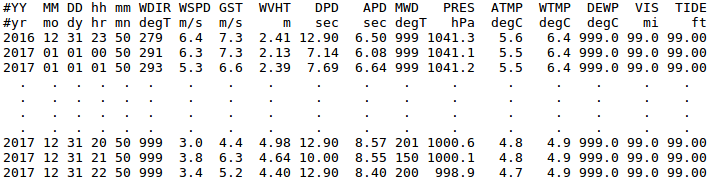
\includegraphics[scale=0.56]{figures/FigureFragmentAnnualTextFile.png}
				\caption{A fragment of an annual text file of the \textit{Station 46001}.}
				\label{fig:fragmentAnnualTexFile}
			\end{figure}
			
			\begin{table}[!ht]
			
				\caption{Measurements descriptions and units of each meteorological variable or attribute collected by the buoys (a detailed description can be found in NDBC website \cite{NOAA_4})}.
				\label{tab:measurementsDescription}
				\footnotesize
				\centering
				
				\begin{tabular}{ccm{7.0cm}@{\setlength{\tabcolsep}{0pt}}m{0.0cm}}
				
					\cline{1-4}
					
					\textbf{Attribute}&\textbf{Units}&\textbf{Description}&\\[0.30cm]
 
					\cline{1-4}
					
					WDIR & degT & The direction the wind is coming from true North. \\
					
					\cellcolor{gray090}WSPD & \cellcolor{gray090} m/s & \cellcolor{gray090} The speed of the wind. \\
					
					GST &  m/s & Peak of gust speed. \\
					
					\cellcolor{gray090} WVHT & \cellcolor{gray090} m & \cellcolor{gray090} Significant wave height. \\
					
					DPD & sec & Dominant wave period (maximum wave energy). \\
					
					\cellcolor{gray090}APD & \cellcolor{gray090} sec & \cellcolor{gray090} Average wave period of all waves. \\
					
					MWD & degT & The direction from which the waves at the dominant period are coming. \\
					
					\cellcolor{gray090}PRES & \cellcolor{gray090} hPa & \cellcolor{gray090} Sea level pressure. \\
					
					ATMP & degC & Air temperature. &\\[0.10cm]
					
					\cellcolor{gray090}WTMP & \cellcolor{gray090} degC & \cellcolor{gray090} Sea surface temperature.\\
					
					DEWP & degC & Dewpoint temperature. \\
					
					\cellcolor{gray090}VIS & \cellcolor{gray090} nmi & \cellcolor{gray090} Visibility of the station. \\
					
					TIDE & ft & The water level. \\
					
					\cline{1-4}
						
				\end{tabular}
			 
			\end{table}
			
			Note that the data collected by the network of buoys may be incomplete due to diverse circumstances such as the weather conditions in which the buoys have to operate, failures or malfunctioning elements of the buoys, among others. Accordingly, it may be the situation that some of the measurements are completely missing (missing date or instance) or partially missing (some measurements not recorded), by a buoy or by a set of buoys, once in a while or over a period of time. It may be also possible that the measurements have been recorded at a time different from the expected one. These aspects have to be taken into account when creating the datasets. This casuistry is explained in detail in Appendix \ref{app:AppendixA}.
			
			\item NNRP provides three-dimensional global reanalysis of numerous meteorological observations (e.g. components  \textit{Zonal} and \textit{Meridional} of the velocity of the wind, relative humidity, pressure, etc.), which is available monthly, daily and every $6$ hours at $00$ Z (Zulu time), $06$ Z, $12$ Z and $18$ Z from $1948$ on a global $2.5\degree$ x $2.5\degree$ grid. Weather observations are from different sources, such as ships, satellites and radar, among others. Reanalysis data is created assimilating such observations employing the same climate model along the whole period of reanalysis in order to decrease the impact of modelling changes on climate statistics. Such information has become a substantial support of the needs of the research community, even more in locations where instrumental (real time) data is not available.
			
			The reanalysis data is available in the NNRP website \cite{NNRP}, which it is accessible through different sections. Such data can be fully (a global $2.5\degree$ x $2.5\degree$ grid) or partially (only the desired reanalysis nodes or sub-grid) downloaded as \textit{Network Common Data Form} (NetCDF) files \cite{NetCDF}, a special binary format for representing scientific data, which provides a description of the file contents and also includes the spatial and temporal properties of the data. Each reanalysis file contains the values of a meteorological variable estimated by a mathematical model for each reanalysis node. For the sake of clarity, in Fig. \ref{fig:subGrid}, an example to approximately illustrate a sub-grid containing six nodes of reanalysis surrounding the geographic localisation of a buoy (obtained from NDBC) is shown.
			
			\begin{figure}[ht!]
				\centering
				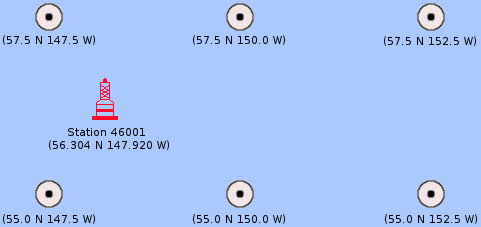
\includegraphics[scale=0.55]{figures/FigureSubGrid.jpg}
				\caption{Sub-grid representation of six nodes of reanalysis surrounding the \textit{Station 46001}.}
				\label{fig:subGrid}
			\end{figure}
			
		\end{itemize}
		
		Therefore, with both sources of information, which complement each other, and carrying out a matching process, SPAMDA will create datasets for prediction tasks. In this way, the dataset input variables will be one or more reanalysis variables from NNRP and one or more measurements from NDBC. The dataset output variable will always be one measurement from NDBC.
		
	\section{SPAMDA}\label{sec:SPAMDA}
		
		SPAMDA combines  meteorological information from NDBC and NNRP to obtain new datasets for oceanic and atmospheric studies. In order to do so, SPAMDA manages three different types of datasets which are described in the following sections, but are briefly introduced bellow for giving the reader a better general understanding:
			\begin{itemize}
				\item \textit{Intermediate datasets}: They contain the meteorological observations from NDBC.
				\item \textit{Pre-processed datasets}: They are obtained as a result of pre-processing tasks performed on the intermediate datasets.
				\item \textit{Final datasets}: Created by merging an intermediate or pre-processed dataset (which contain the information from NDBC) with the reanalysis data from NNRP. This procedure is referenced in SPAMDA as matching process and will be carried out according to the study to be performed (classification or regression).
			\end{itemize}
		
		\begin{figure}[ht!]
			\centering
			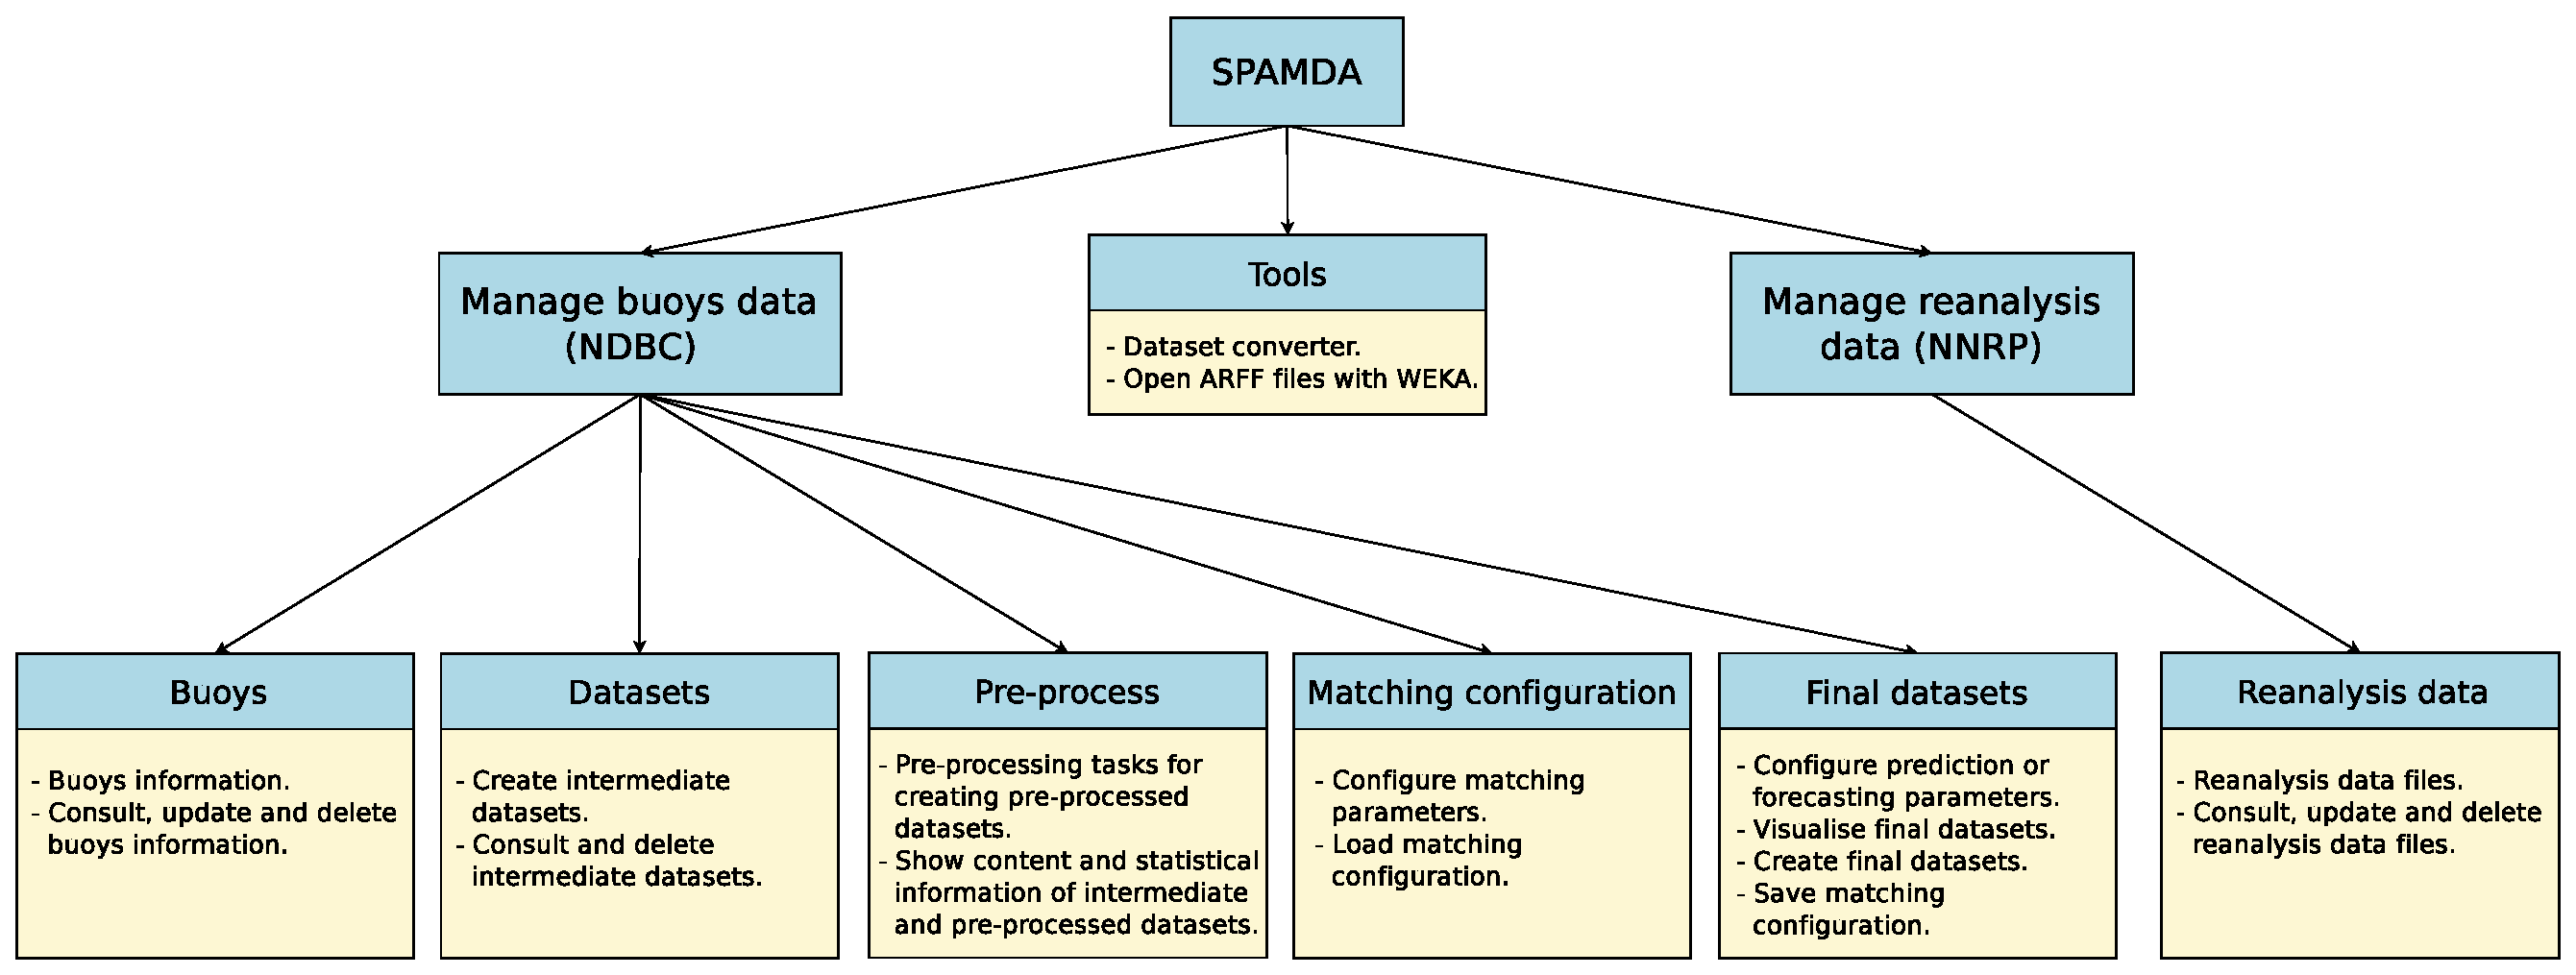
\includegraphics[scale=0.33]{figures/FigureSPAMDA.eps}
			\caption{Brief outline of the functionality provided by SPAMDA.}
			\label{fig:SPAMDA}
		\end{figure}
		SPAMDA consists of three main functional modules, whose main features, represented in Fig. \ref{fig:SPAMDA}, are the following:
		\begin{itemize}
			
			
			\item \textit{Manage buoys data}: The aim of this module is to provide features for the management and analysis of the information related to the buoys from NDBC. This includes:
			\begin{enumerate}
				\item Entering and updating the information of each buoy.
				\item Creation of intermediate datasets with the collected measurements.
				\item Pre-processing tasks for obtaining the pre-processed datasets.
				\item Matching process to merge the information from NDBC and NNRP.
				\item Creation of the final datasets accordingly to the ML technique to use (classification or regression).
			\end{enumerate}
			
			\item \textit{Manage reanalysis data}: This module is used for the management of the reanalysis data provided by the NNRP. In this way, researchers can keep the reanalysis data files updated for their studies. Such files will be used, depending on researchers needs, in the matching process when obtaining the final datasets.
			
			\item \textit{Tools}: This module includes features for converting intermediate or pre-processed datasets to ARFF or CSV format and for opening ARFF files with WEKA software.
			
		\end{itemize}

		In the following subsections each integrated functional module is described in detail.

			\subsection{Buoys}\label{sec:Buoys}
			
				When a new buoy is included in SPAMDA the following information, which can be obtained from NDBC, is requested:
				\begin{itemize}
					\item \textit{Station ID}: An alphanumeric identifier that allows easy identification of the buoy.
					\item \textit{Description}: A short description of the buoy.
					\item \textit{Latitude}: North or South geographical localisation (degrees) of the buoy.
					\item \textit{Longitude}: West or East geographical localisation (degrees) of the buoy.
					\item \textit{Measurements files}: The above-mentioned annual text files of the standard meteorological information recorded by the buoy and downloaded from the NDBC website. This will be used for the creation of the intermediate datasets. One file per year is expected.
				\end{itemize}
				
				For clarification, an example is presented in Fig. \ref{fig:buoys}, where the buoy ID1 has three annual text files and the buoy ID2 has two annual text files.
				
				\begin{figure}[ht!]
					\centering
					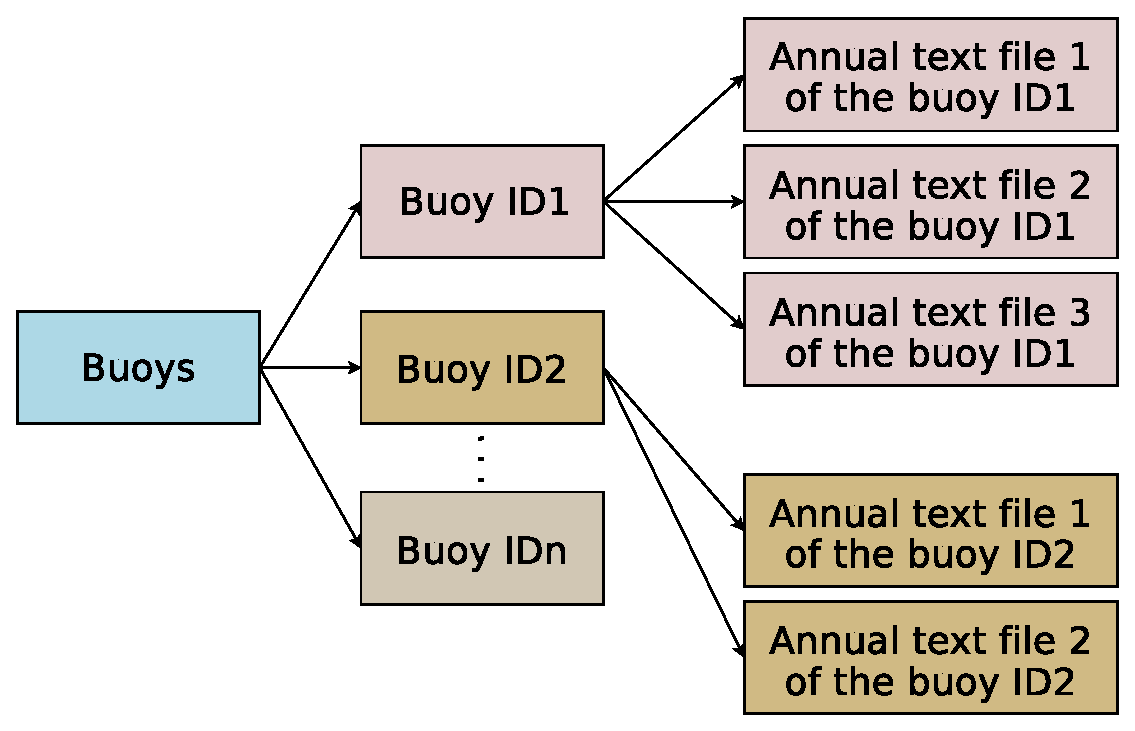
\includegraphics[scale=0.4]{figures/FigureBuoys.eps}
					\caption{Example of entering two buoys with its annual text files.}
					\label{fig:buoys}
				\end{figure}


			\subsection{Datasets}\label{sec:Datasets}
			
				Once a buoy has been included as described in Section \ref{sec:Buoys}, it is possible to create datasets with one or more annual text files, which are referenced in SPAMDA as intermediate datasets. In this module, researchers can manage intermediate datasets of each buoy, which are the baseline for their studies, by creating new ones or deleting the unnecessary ones.
				
				When an intermediate dataset is created, it is associated with its corresponding buoy. Besides, a summary of its content is also created, providing relevant information such as the number of instances, the dates of the first and last measurements, the annual text files included, and the missing and duplicated dates.
				
				An example where three intermediate datasets have been created is presented in Fig. \ref{fig:datasets}. The two intermediate datasets of the buoy ID1 contain meteorological data of different years, and the intermediate dataset of the buoy ID2 contains meteorological data of two years. For each buoy, as many intermediate datasets as needed can be created.
				
				\begin{figure}[ht!]
					\centering
					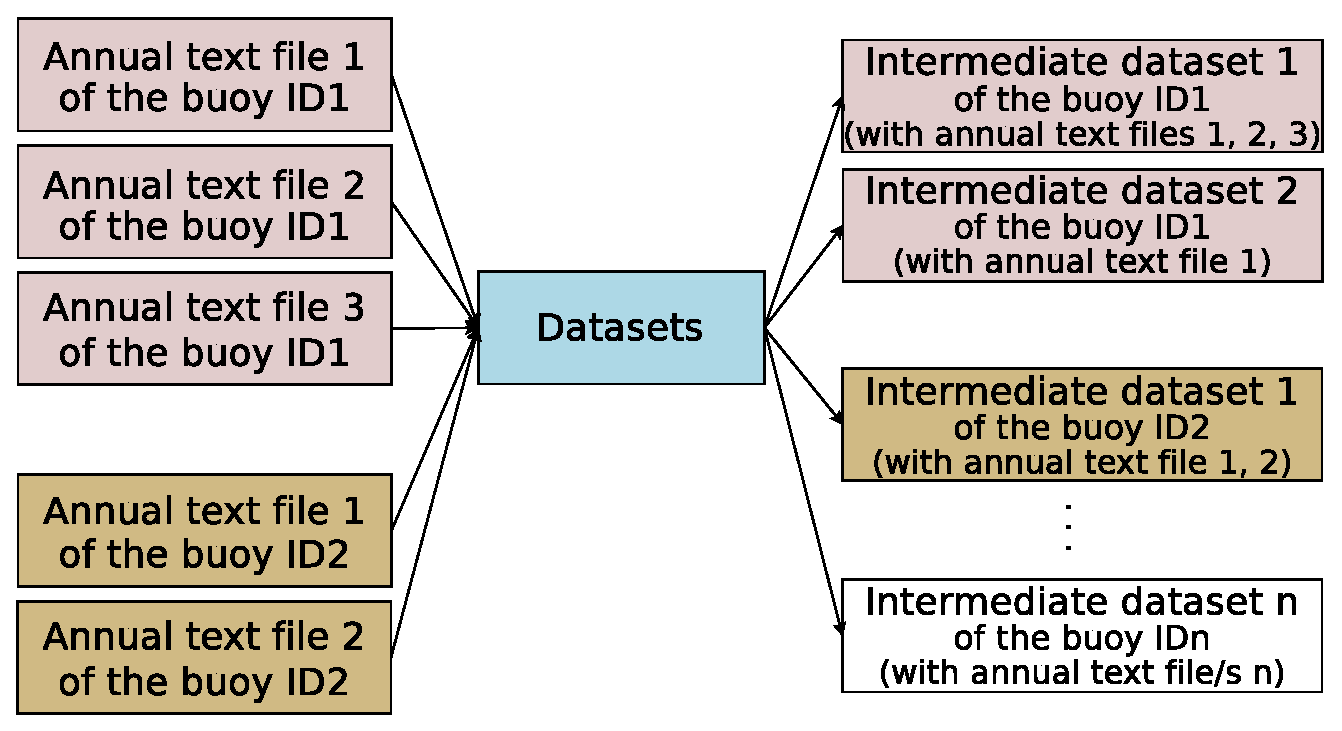
\includegraphics[scale=0.40]{figures/FigureDatasets.eps}
					\caption{Example of the creation of the intermediate datasets.}
					\label{fig:datasets}
				\end{figure}
				
				
			\subsection{Pre-process} \label{sec:Preprocess}
				
				Data pre-processing prepares the raw data (intermediate datasets) to be able to be treated correctly by ML algorithms. This action can enhance the quality of data before the learning phase, by applying pre-processing tasks (filters). The result will be referenced as pre-processed datasets.
				
				SPAMDA provides several filters grouped in three categories, \textit{Attribute}, \textit{Instance} and \textit{Recover missing data}, including the configuration of their parameters and a short description of them:
				
				\begin{itemize}

				 \item \textit{Attribute}: All theses filters can be applied to the attributes (variables of the buoy from NDBC) of the intermediate dataset.
				 
					\begin{itemize}
						\item \textit{Normalize}: This filter normalises all numeric values of each attribute. The resulting values are by default in the interval [0,1].
						\item \textit{Remove}: It removes an attribute or a range of them.
						\item \textit{RemoveByName}: It removes attributes based on a regular expression matched against their names.
						\item \textit{ReplaceMissingValues}: For each attribute, all the missing values will be replaced by the average value of the attribute.
						\item \textit{ReplaceMissingWithUserConstant}: This filter replaces all the missing values of the attributes with an user-supplied constant value.
					\end{itemize}
				 
				 \item \textit{Instance}: All theses filters can be applied to the instances (hourly measurements of the buoy from NDBC) of the intermediate dataset.
					\begin{itemize}
						\item \textit{RemoveDuplicates}: With this filter, all duplicated instances are removed.
						\item \textit{RemoveWithValues}: This filter removes all the instances that match the attribute and the value supplied by the user.
						\item \textit{SubsetByExpression}: It removes all the instances which do not match a user-specified expression.
					\end{itemize}
				 
				 \item \textit{Recover missing data}: All these filters can be applied to the instances of the intermediate dataset.
					\begin{itemize}
						\item \textit{Replace missing values with next nearest hour}: The missing values of each attribute are replaced with the next nearest non missing value.
						\item \textit{Replace missing values with previous nearest hour}: This filter replaces the missing values of each attribute with the previous nearest non missing value.
						\item \textit{Replace missing values with next $n$ hours mean}: The missing values of each attribute are replaced with the next $n$ nearest non missing values mean, where $n$ can be configured by the user.
						\item \textit{Replace missing values with previous $n$ hours mean}: This filter replaces the missing values of each attribute in the intermediate dataset with the previous $n$ nearest non missing values mean.
						\item \textit{Replace missing values with symmetric $n$ hours mean}: The missing values of each attribute in the intermediate dataset are replaced with the $n$ previous and $n$ next non missing values mean.
					\end{itemize}
				 
				\end{itemize}
				
				SPAMDA allows researchers to undo the last filter applied or to restore the initial content of the intermediate dataset. Besides, the content and relevant statistical information of the intermediate and the pre-processed datasets can be visualised in this module, for example: minimum and maximum values, mean, standard deviation or even the number of instances with missing values.
				
				Fig. \ref{fig:preprocess} shows an example where the intermediate datasets 1 and 2 of the buoy ID1 have been pre-processed, obtaining as a result the pre-processed dataset 1 of each one. The intermediate dataset 1 of the buoy ID2 has been also pre-processed. \textit{Pre-processed dataset n} represents that researchers can create as many pre-processed datasets as they consider opportune.
				
				\begin{figure}[ht!]
					\centering
					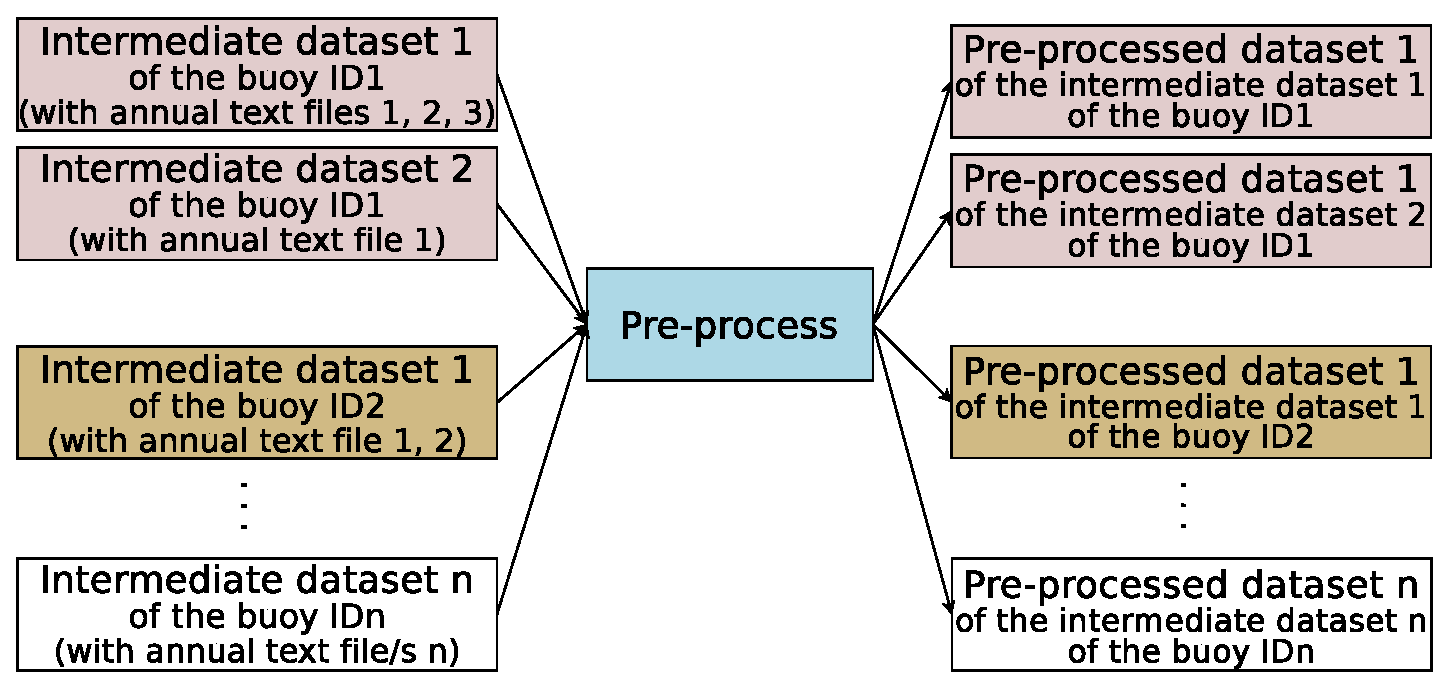
\includegraphics[scale=0.40]{figures/FigurePreprocess.eps}
					\caption{Example of the creation of pre-processed datasets.}
					\label{fig:preprocess}
				\end{figure}
				
				Nevertheless, further pre-processing tasks can be performed after obtaining the final datasets by means of the Explorer environment of WEKA or other tools.
				
				
			\subsection{Matching configuration}
			\label{sec:matching_conf}
			
				The automatic integration of the data provided by the two sources of information described in Section \ref{sec:DataSources}, to merge and format such data, is denominated as the matching process in this document. Such process is one of the most powerful and remarkable features of this software tool due to its great relevance and extensive casuistry. In this sense, SPAMDA has been developed to provide great flexibility to researchers.
				
				The matching procedure is performed using an intermediate or pre-processed dataset, which includes the measurements collected by a buoy from NDBC, and the needed reanalysis data files from NNRP. Note that SPAMDA is able to manage the NetCDF binary format for handling the information stored in the reanalysis files.
				
				Such process merges the information of both sources that match on time, but, given that the reanalysis data is available with a minimum time horizon of $6$ hours at $00$ Z, $06$ Z, $12$ Z and $18$ Z, and the measurements of the buoys are recorded at hourly intervals, from $00$:$50$ to $23$:$50$ UTC, the matching can only be carried every $6$ hours (discarding the rest of measurements from the buoy data). Besides, and since there is still a difference of 10 minutes, the matching with the reanalysis data will be performed with the nearest buoy measurement (before or after) within a maximum of 60 minutes of difference. Finally, the matched instances of both sources will form the final datasets.
				
				Fig. \ref{fig:matchingProcess} presents an example of matching with the measurements collected during $2017$ by \textit{Station 46001} (NDBC) and the reanalysis data (NNRP) of the variable \textit{pressure} for reanalysis nodes $57.5$ N $\times$ $147.5$ W and $55.0$ N $\times$ $147.5$ W in the same year. In this way, only the instances from both sources that are linked with arrows (highlighted in green colour) will be used in the creation of the final datasets. Although the reanalysis dates have been presented in a human readable format, note that reanalysis dates are stored in hours from $01$-$01$-$1800$, and they have to be transformed for comparison taking into account the time zone. Such transformation is automatically done by SPAMDA when matching the instances.
				
				The reader can check in Appendix \ref{app:AppendixA} an example with a more complex case of the procedure.
				\begin{figure}[ht!]
					\centering
					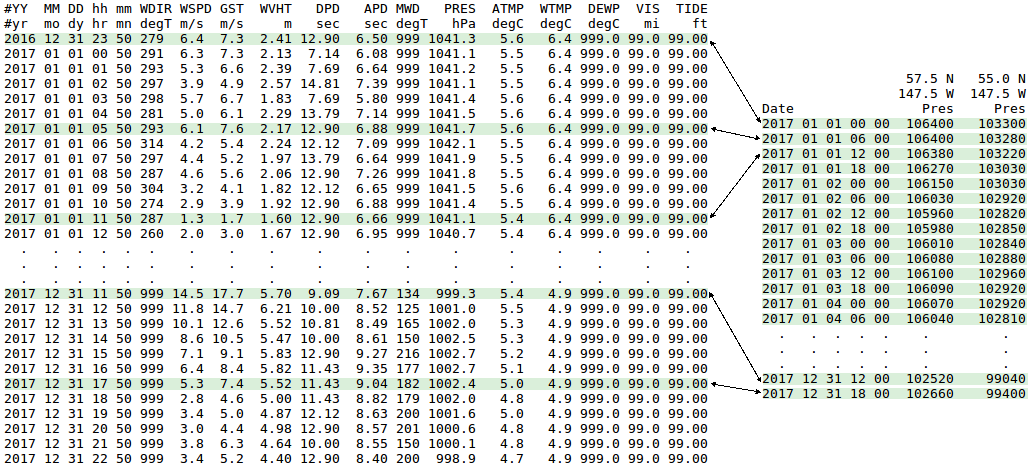
\includegraphics[scale=0.43]{figures/FigureMatchingProcess.png}
					\caption{An example of matching the data from NDBC (left) and NNRP (right).}
					\label{fig:matchingProcess}
				\end{figure}
				
				SPAMDA allows researchers to perform a customisable matching process, for obtaining as many different versions of the same meteorological data as needed.
				Prediction tasks are based on the estimation of the output attribute using the information provided by the input attributes. Depending on the task, the datasets must be prepared and configured differently:
				\begin{itemize}
					\item \textit{Classification}: The final datasets will be ready to use as input for ML classifiers, requiring a nominal output attribute, whose specific preparation is detailed in Section \ref{sec:FinalDatasets}.
					\item \textit{Regression}: The final datasets will be ready to use as input for regression methods, requiring a real output attribute, whose preparation is also explained in Section \ref{sec:FinalDatasets}.
					\item \textit{Direct matching}: In this case the inputs attributes have a direct correspondence with the output attribute, and it is not necessary to perform any additional preparation. Both input and target attributes are synchronised in time, in such a way that the final dataset is not intended for prediction purposes. For example, the final datasets may be used in lost data recovering tasks, in correlation studies, in descriptive analyses, etc.
				\end{itemize}
				
				The following parameters can be specified for the matching process:
				\begin{itemize}
				
					\item \textit{Flux of energy} \cite{FERNANDEZ201544}: When the $F_e$ is selected, it will be used as output. This attribute is not collected by the buoys, but there are two parameters from which it can be computed: $H_s$ and $T_e$, which are collected as WVHT and APD attributes, respectively, and were described in Table \ref{tab:measurementsDescription}. In this way, SPAMDA obtains the $F_e$ (measured in kilowatts per meter) of each instance using the following equation:
					\begin{equation}
							F_e = 0.49 \cdot H^2_s \cdot T_e,
							\label{eq:fluxOfEnergy}
					\end{equation}
						
					where $H_s$ is measured in meters and $T_e$ in seconds. $F_e$ is referred to as flux of energy but it is defined as an average energy flux because $H_s$ is an average wave height (see descriptions of the measurements on the NDBC website).
					
					\item \textit{Attribute to predict}: Instead of using $F_e$, researchers can select any of the attributes collected by the buoys as output (e.g. significant wave height, WVHT, wind direction, WDIR, sea level pressure, PRES, etc.). Therefore, they can conduct different studies by selecting one attribute or other.

					\item \textit{Reanalysis data files}: In order to have a possible better description of the problem under study, more than one reanalysis variable can be considered as input. Remember that these files have to be previously downloaded from the NNRP website \cite{NNRP}, which should set the range of dates (temporal properties) and the desired sub-grid (spatial properties, see Fig. \ref{fig:subGrid}) for each variable of reanalysis.
					
					In that sense, the reanalysis data files must have the same spatial and temporal properties but related to different variables. SPAMDA simplifies this task by showing the reanalysis data files that are compatibles each other, and checking that the selection made by the researches meets that condition.
					
					\item \textit{Buoys attributes}: In addition to the reanalysis variables, the final datasets will also include the selected attributes as inputs (of the intermediate or pre-processed dataset used), providing a possible better characterisation of the problem under study, although it will depend on how correlated the attributes are.

					\item \textit{Include missing dates}: As above-mentioned, the information collected by a buoy may be incomplete due to measurements not recorded by it. As a consequence, the matching of instances between both sources of information may not be possible (missing dates). In that situation, researchers can consider two options: 1) discard the instances affected or 2) include them. In the latter case, the final datasets will contain the affected instances, but the measurements of the buoy will be stored as missing values in WEKA format, denoted as \guillemotleft\textit{?}\guillemotright.
					
					\item \textit{Nearest reanalysis nodes to consider}: As already shown in Fig. \ref{fig:subGrid} (which represents six reanalysis nodes), the reanalysis data files may contain information of several reanalysis nodes. In this way, researchers can:
					
						\begin{itemize}
							
							\item Consider all the reanalysis nodes contained in each file: in this case, the information provided by each reanalysis node contained in each selected reanalysis data file will be used.
							
							\item Consider only some of the reanalysis nodes contained in each file: in this case, the information used is only that corresponding to the closest nodes to the buoy (the number of nodes, $N$, is indicated by the user). To do that, SPAMDA uses the \textit{Haversine} equation \cite{Haversine_2009} (or the great-circle distance) to calculate the distance from the location of the buoy to each node of reanalysis and obtain the closest ones. Haversine equation performs calculation from main point to destination point with a trigonometric function:
								\begin{eqnarray}
									\label{eq:Haversine}
									d(p_0,p_j) & = & \arccos(\sin(lat_0)\cdot \sin(lat_j) \nonumber \\
									& & \cdot \cos(lon_0-lon_j) + \cos(lat_0) \\
									& & \cdot \cos(lat_j)), \nonumber 
								\end{eqnarray}
							where $p_0$ is the geographical location of the buoy and $p_j$ is the position of each node. Finally, $lat$ and $lon$ represent the latitude and longitude of the positions of the points.
						\end{itemize}
					
					\item \textit{Number of final datasets}: Depending on the number of nearest reanalysis nodes to consider, the number of final datasets to create and the content of them can be configured according to the following options:
						\begin{itemize}
						
							\item \textit{One (using weighted mean of the $N$ nearest reanalysis nodes)}: Only one final dataset will be created, which will contain the attributes (the selected one as output and the selected ones as inputs) of the intermediate or pre-processed dataset used, along with a weighted mean of each variable of the reanalysis data used (one per selected reanalysis data file). This weighted mean is obtained by SPAMDA and uses Eq. \ref{eq:Haversine} to calculate the distance from the geographical position of the buoy to each node of reanalysis. Once the distances have been computed, they are normalised and inverted as shown in the following equation:
								\begin{linenomath*}
									\begin{equation}
										w_i=\frac{d(p_0,p_i)}{\sum_{j=1}^{N} d(p_0,p_j)}, ~~i=1, \ldots, N.
										\label{eq:weightedMean}
									\end{equation}
								\end{linenomath*}

							Then, with these calculated weights, a weighted mean of each variable of reanalysis is obtained for each of the $N$ nodes. In this way, the closest reanalysis nodes to the geographical position of the buoy will provide more information.
							
							Considering as example the two nearest reanalysis nodes represented in Fig. \ref{fig:subGrid} and the reanalysis variables air temperature and pressure, the weighted mean of each reanalysis variable will be calculated using the reanalysis nodes $57.5$ N $\times$ $147.5$ W and $55.0$ N $\times$ $147.5$ W.
							
							\item \textit{'N' (one per each reanalysis node)}: As many final datasets as the number of nearest $N$ reanalysis nodes configured by researcher will be created. Therefore, each final dataset will contain the value of each reanalysis variable used of the nearest corresponding reanalysis node, along with the selected attributes of the intermediate or pre-processed dataset used. In this way, researchers can perform comparison studies depending on the reanalysis node considered, to achieve better performance for the problem under study.
							
							In this case, and considering as example the four closest reanalysis nodes (see Fig. \ref{fig:subGrid}) and the reanalysis variables air temperature and pressure, four final datasets will be created, containing each one the information of both reanalysis variables of the corresponding reanalysis node: $57.5$ N $\times$ $147.5$ W, $55.0$ N $\times$ $147.5$ W, $57.5$ N $\times$ $150.0$ W and $55.0$ N $\times$ $150.0$ W, along with the selected attributes of the intermediate or pre-processed dataset used.
							
						\end{itemize}
					
				\end{itemize}
						
				Once the matching parameters have been described, for a better understanding of them,  Fig. \ref{fig:directMatching} presents an example of the data integration considering the data shown in Fig. \ref{fig:matchingProcess} and using the following configuration\footnote{Note that the date is shown just for a better understanding, but it will not be included in the final dataset.}:
					\begin{itemize}
						\item Attribute to predict: variable WVHT (Fig. \ref{fig:directMatchingWave}) / flux of energy (Fig. \ref{fig:directMatchingFlux}).
						\item Variable Pres as reanalysis input attribute.
						\item Variable WSDP as buoy input attribute.
						\item Not including missing dates.
						\item Considering the closest reanalysis node.
						\item Task to be used: \textit{Direct matching}.
					\end{itemize}

				\begin{figure}[ht!]
					\centering
					\subfloat[attribute to predict: WVHT\label{fig:directMatchingWave}]{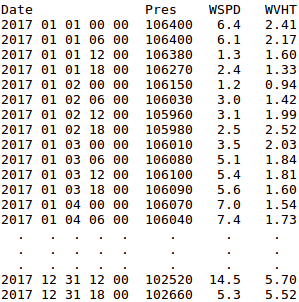
\includegraphics[width=0.4\textwidth]{figures/FigureDirectMatching.png}}\hfill
					\subfloat[attribute to predict: flux of energy\label{fig:directMatchingFlux}]{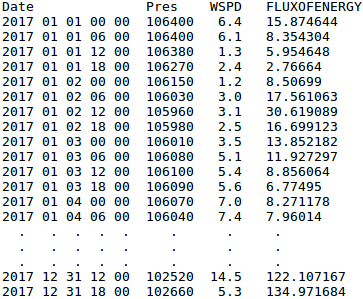
\includegraphics[width=0.47\textwidth]{figures/FigureDirectMatching_EF.png}}\hfill
					\caption{Example of data integration for \textit{Direct matching}.} \label{fig:directMatching}
				\end{figure}
				
			\subsection{Final datasets} \label{sec:FinalDatasets}

				Once the matching process has been performed with the desired configuration, it is necessary to prepare the matched information for the desired prediction task (\textit{Regression} or \textit{Classification}), obtaining as a result the final datasets. Remember that \textit{Direct matching}, as it was described in Section \ref{sec:matching_conf}, performs a direct correspondence between the attributes used as inputs and the output one, and it is not necessary to carry out any preparation.
				
				SPAMDA allows researchers to make such preparation by means of the following options:
				
					\begin{itemize}

						\item \textit{Prediction horizon} (Classification and Regression): This option indicates the time gap for moving backward the attribute to predict (output attribute). In this way, the input attributes (variables of the buoy and reanalysis data) will be used to predict the output attribute in a specific future time (e.g. +6h, +12h, +18h, +1 day, etc.).
						
						The minimum interval for increasing and decreasing the prediction horizon is $6$h (due to reanalysis data temporal resolution) \cite{DORADOMORENO2017428}, the same interval used when the matching process is carried out. Therefore, for each increment of the prediction horizon, an instance of the dataset is lost (as this future information is not available). As the minimum prediction horizon is $6$h, at least one instance will be lost. The relation between the inputs and the output (attribute to predict) is defined as follows:
						\begin{linenomath*}
							\begin{equation}
								o_{t+\Delta t}=\phi(\mathbf{b}_t,\mathbf{r}_{t}),
								\label{eq:noSynchronisingRD}
							\end{equation}
						\end{linenomath*}
						where $t$ is the time instant to study, $\Delta t$ is the prediction horizon, $o$ is the attribute to be predicted, $\mathbf{b}_t$ represents the vector that contains the selected NDBC variables, and, finally, $\mathbf{r}_t$ represents the vector that contains the selected reanalysis variables. In this way and considering the matched information shown in Fig. \ref{fig:directMatchingWave}, WVHT is $o$, the vector $\mathbf{b}$ contains the variable WSPD and the vector $\mathbf{r}$ contains Pres.
						
						Optionally, the reanalysis variables can be synchronised with the attribute to predict. Given that these variables are estimated by a mathematical model, we can obtain very good future estimations, which can improve the performance of the results. In this case, the relation between the inputs and the attribute to predict would be:
						\begin{linenomath*}
							\begin{equation}
								o_{t+\Delta t}=\phi(\mathbf{b}_t,\mathbf{r}_{t+\Delta t}).
								\label{eq:synchronisingRD}
							\end{equation}
						\end{linenomath*}
						
						Note that the selected NDBC variables as input cannot be synchronised with the attribute to predict.
						
 						For the sake of clarity, considering the matched information shown in Fig. \ref{fig:directMatchingWave}, an example of building a dataset for a \textit{Regression} task is shown in Fig. \ref{fig:regressionNoSync}. As mentioned earlier, this prediction task requires a real output variable (in this case, WVHT, the last one). The options considered for the preparation of each final dataset are the following:
 							\begin{itemize}
 								\item Do not synchronise the reanalysis data (see Eq. \ref{eq:noSynchronisingRD} for the relation between the inputs and the output).
 								\item A prediction horizon of $6$h.
 							\end{itemize}
							
 						Note that, due to prediction horizon is $6$h, the values of WVHT attribute are moved backward one instance (up). As a consequence, the last instance ($2017$/$12$/$31$ $18$:$00$) is lost and is not included in the final dataset. Besides, and because the reanalysis data has not been synchronised, the values of the Pres and WSPD variables are at the same time instant ($t$ in Eq. \ref{eq:noSynchronisingRD}).
						
 						Moreover, considering again the matched information shown in Fig. \ref{fig:directMatchingWave}, an example of the creation of the same dataset but applying synchronisation (see Eq. \ref{eq:synchronisingRD}) is shown in Fig. \ref{fig:regressionSync}.
						
							\begin{figure}[ht!]
								\centering
								\subfloat[without synchronisation\label{fig:regressionNoSync}]{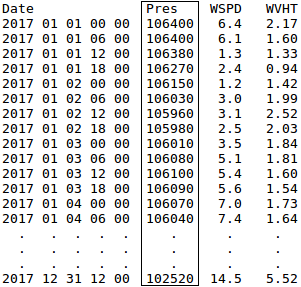
\includegraphics[width=0.39\textwidth]{figures/FigureRegressionNoSync.png}}\hfill
								\subfloat[with synchronisation\label{fig:regressionSync}]{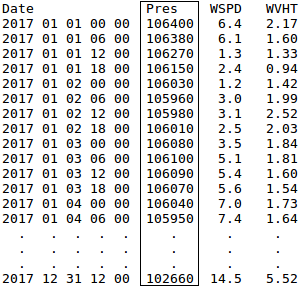
\includegraphics[width=0.39\textwidth]{figures/FigureRegressionSync.png}}\hfill
								\caption{Example of the creation of a \textit{Regression} dataset with a prediction horizon of $6$h.} \label{fig:regression}
							\end{figure}

						Again, and due to the prediction horizon selected ($6$h), the values of the WVHT attribute are moved backward one instance (up) and the last instance ($2017$/$12$/$31$ $18$:$00$) is not included in the final dataset. But now, the values of the Pres variable are also moved backward one instance (due to the synchronisation). Therefore, in this case, Pres is at the same time instant as the attribute to predict (${t+\Delta t}$ in Eq. \ref{eq:synchronisingRD}).
						
						\item \textit{Thresholds of the output attribute} (Classification): Since the values of the variables collected by the buoys are real numbers, it is necessary to discretise them (convert them from real to nominal values) for the attribute selected as output (attribute to be predicted). SPAMDA allows researchers to perform this process by defining the necessary classes with their thresholds, which will be used to carry out such discretisation.
						
						Considering again the matched information shown in Fig. \ref{fig:directMatchingWave}, an example of the creation of a \textit{Classification} dataset is shown in Fig. \ref{fig:prediction}. The options considered for the preparation of the final dataset are the following:
							\begin{itemize}
								\item Do not synchronise the reanalysis data.
								\item A prediction horizon of $6$h.
								\item The thresholds shown in Table \ref{tab:thresholds}.
							\end{itemize}
							
						\begin{table}[!h]
						
							\caption{Thresholds for the classification example represented in Fig. \ref{fig:prediction}}
							\label{tab:thresholds}
							\footnotesize
							\centering

							\begin{tabular}{cm{3.20cm}cc@{\setlength{\tabcolsep}{0pt}}m{0.0cm}}
							
								\cline{1-5}
								
								\textbf{Class}&\textbf{Description}&\textbf{Lower end [}&\textbf{Upper end )}&\\[0.20cm]
			
								\cline{1-5}
								
								Low & Low wave height & $0.36$ & $1.5$&\\[0.15cm]
								
								\cellcolor{gray090}Average & \cellcolor{gray090}Average wave height & \cellcolor{gray090}$1.5$ & \cellcolor{gray090}$2.5$&\\[0.15cm]
								
								Big & Big wave height & $2.5$ & $4.0$&\\[0.15cm]
								
								\cellcolor{gray090}Huge & \cellcolor{gray090}Huge wave height & \cellcolor{gray090}$4.0$ & \cellcolor{gray090}$9.9$&\\[0.15cm]

								\cline{1-5}
									
							\end{tabular}
						
						\end{table}

							
						\begin{figure}[ht!]
							\centering
							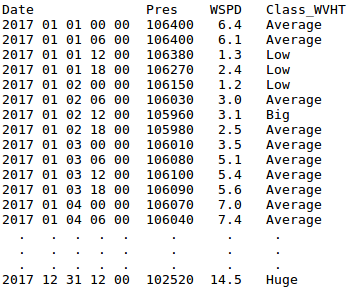
\includegraphics[scale=0.6]{figures/FigureClassification.png}
							\caption{An example of the creation a \textit{Classification} dataset, with a prediction horizon of $6$h and without synchronisation.}
							\label{fig:prediction}
						\end{figure}
						
						Note that the attribute to be predicted has been renamed to \textit{Class\_WVHT} to show that it is now a nominal variable, because its values have been discretised according to the thresholds (usually defined by an expert). Besides, and due to the $6$h prediction horizon, the last instance is lost ($2017$/$12$/$31$ $18$:$00$) and the values of the attribute \textit{Class\_WVHT} are moved backward one instance (up). As the reanalysis data have not been synchronised, the values of the Pres and WSPD variables are at the same time instant ($t$ in Eq. \ref{eq:noSynchronisingRD}).
						
					\end{itemize}
				
				The content of the final datasets, obtained as the result of the preparation of the matched data, can be visualised to check everything before saving them on disk. Such preparation can be performed as many times as required and considering the different options in each moment. Although the date will not be included in the final datasets, it can be shown to properly check the matching.
				
				Finally, it is necessary to define the output configuration to create the final datasets:			
				\begin{itemize}

					\item \textit{Output path file}: Name of the final datasets and folder to save them on disk.
						
					\item \textit{Final datasets format}:

						\begin{itemize}
						
							\item \textit{ARFF}: \textit{Attribute-Relation File Format} \cite{WEKA_ARFF}, which is used by WEKA. SPAMDA allows researchers to directly open the final datasets in the Explorer environment of WEKA (in the same context of work), enabling them to choose the most appropriate ML method to tackle the problem under study.

							\item \textit{CSV}: \textit{Comma-Separated Values}. This format is included in order to consider other different tasks of software tools.
							
						\end{itemize}
					
				\end{itemize}
				
				A text file that summarises the configuration used in matching process and in the preparation of the matched data is also generated. It can be saved and loaded, enabling researchers to resume their studies at any other time.
				
				
			\subsection{Manage reanalysis data}
				
				As mentioned in Section \ref{sec:DataSources}, the reanalysis data files provided by NNRP contain the estimated values by a mathematical model of one meteorological variable.
				
				In this module (see Fig. \ref{fig:SPAMDA}), SPAMDA includes features for entering new files and deleting the unnecessary ones. Besides, useful information about the content of each reanalysis file can be consulted such as name of the file and the reanalysis variable, number of instances and reanalysis nodes, initial and final time, latitude and longitude. All these fields summarise the temporal and spatial properties of the data. Thus, researcher can quickly and easily identify each reanalysis file entered in SPAMDA.
				
				An example where two reanalysis data files have been entered in SPAMDA is shown in Fig. \ref{fig:manageReanalisys}.
				
				\begin{figure}[ht!]
					\centering
					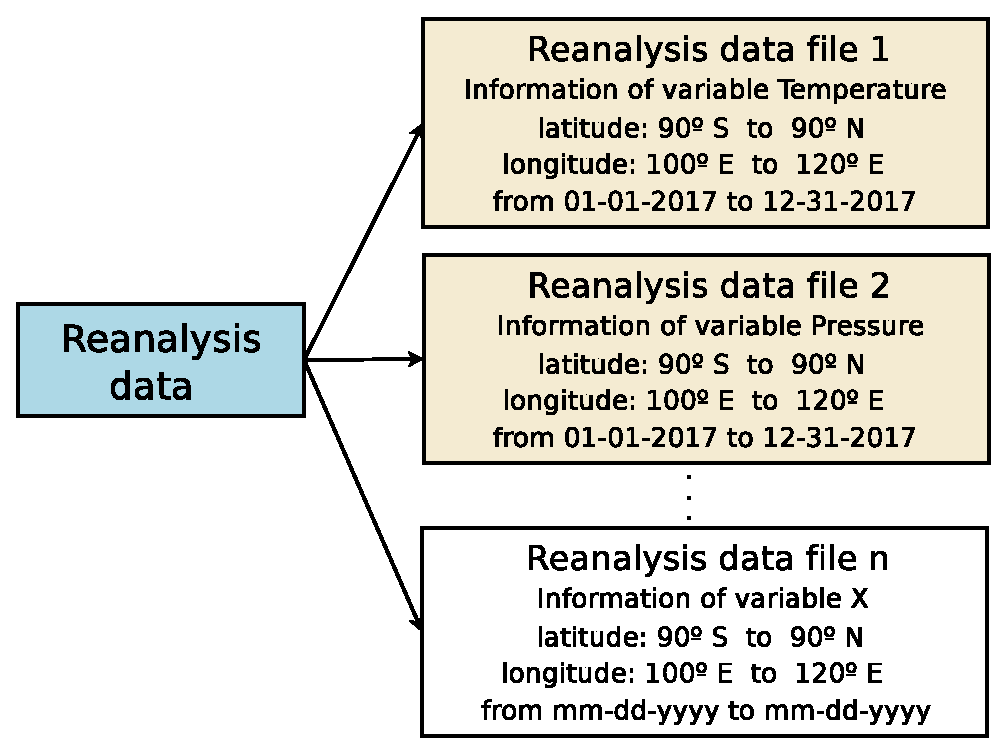
\includegraphics[scale=0.45]{figures/FigureManageReanalisys.eps}
					\caption{Example of entering two reanalysis data files.}
					\label{fig:manageReanalisys}
				\end{figure}
				
			\subsection{Tools}
			
				SPAMDA also contains another module that provides two utilities: one of them is \textit{Dataset converter} used for converting the desired intermediate or pre-processed datasets to ARFF or CSV formats; the other utility can be used for opening ARFF files with WEKA Explorer environment, which is useful for easily checking the results of different configurations of the pre-processing.
				
	\section{A case study applied to Gulf of Alaska}\label{sec:CaseStudy}
		
		This section describes how SPAMDA works in a practical approach showing two examples to create fully processed datasets (final datasets) starting from the raw data. The objective of these final datasets is to be used with SC and ML algorithms for environmental modelling, in this case, to classify waves depending on their height and to predict energy flux in the Gulf of Alaska.
		
		On the one hand, wave classification is addressed as a multi-class approach, given that a continuous attribute can be discretised, using different thresholds, in distinct classes. Such waves modelling can be applied with different purposes, such as missing buoy data reconstruction, extreme significant wave heights detection or decision-making and risk assessment about operational works in the sea.

		On the other hand, the prediction of the energy flux is addressed as a regression problem. Energy flux prediction is related to marine energy and it is useful to characterise the wave energy production from WECs facilities, which could be injected into the electric network or supplied to existing marine platforms.

		\subsection{Gathering the information and introducing it in SPAMDA}\label{sec:ObtainingFinalDataset}
		
			The data collected to perform this case study is:
			\begin{enumerate}
			\item The measurements obtained from 2013 to 2017 by the buoy with ID 46001, placed in the Gulf of Alaska, which are provided by NDBC as annual text files. This data is publicly available at the NDBC website. 
			\item Complementary information collected from reanalysis data containing air temperature (air), pressure (pres) and two components of wind speed measurements, South-North (vwind) and West-East (uwind). This information can be downloaded from the NNRP website in NetCDF format for the four closest nodes of reanalysis surrounding the position of the buoy. Concretely, the closest reanalysis nodes downloaded are $57.5$ N $\times$ $147.5$ W, $57.5$ N $\times$ $150$ W, $55$ N $\times$ $147.5$ W and $55$ N $\times$ $150$ W. However, as will be seen later, only the information from the nearest node will be used in the data integration process.
			\end{enumerate}
		
			After gathering the information described above, researchers can open SPAMDA. In Fig. \ref{fig:main_view}, the main view is shown. In order to input the reanalysis data which will be used in further steps for creating the final dataset, researchers has to select the option \textbf{\textit{Manage reanalysis data}}.

			\begin{figure}[ht]
				\centering
				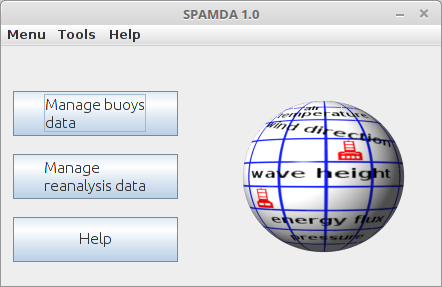
\includegraphics[width=0.5\textwidth]{figures/FigureMain_view.png}
				\caption{SPAMDA main view.}\label{fig:main_view}
			\end{figure}
			
			Then, the view of Fig. \ref{fig:reanalysis} is shown. Here, using the buttons located at the bottom, it is possible to add, delete or consult any data from the different reanalysis files. Once the information has been introduced in the application, this view can be closed and the user can go back to the main view to continue entering the information related to the buoy under study. 
			
			\begin{figure}[ht!]
				\centering
				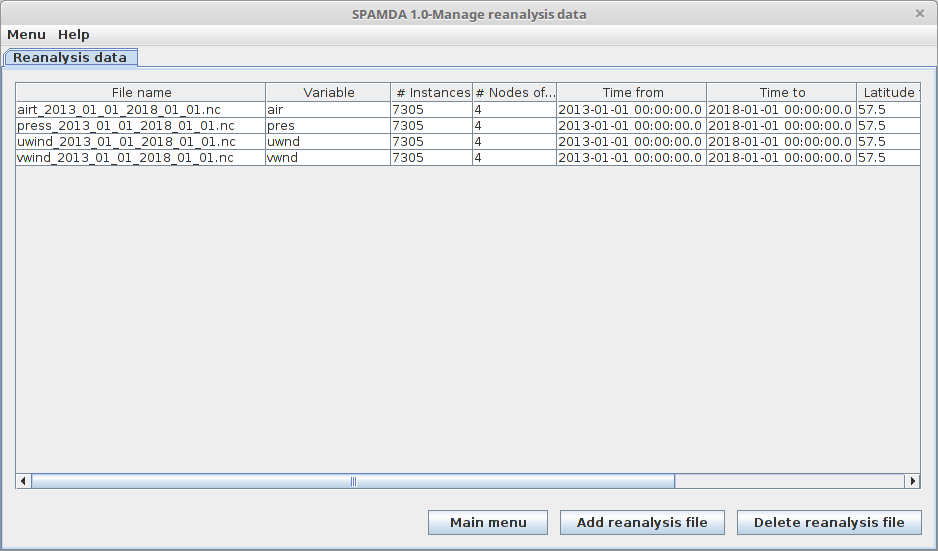
\includegraphics[width=0.89\textwidth]{figures/FigureManage_reanalysis_data.png}
				\caption{\textit{Manage reanalysis data} view: downloaded files containing the four closest reanalysis nodes.}\label{fig:reanalysis}
			\end{figure}
		
			\begin{figure}[ht!]
				\centering
				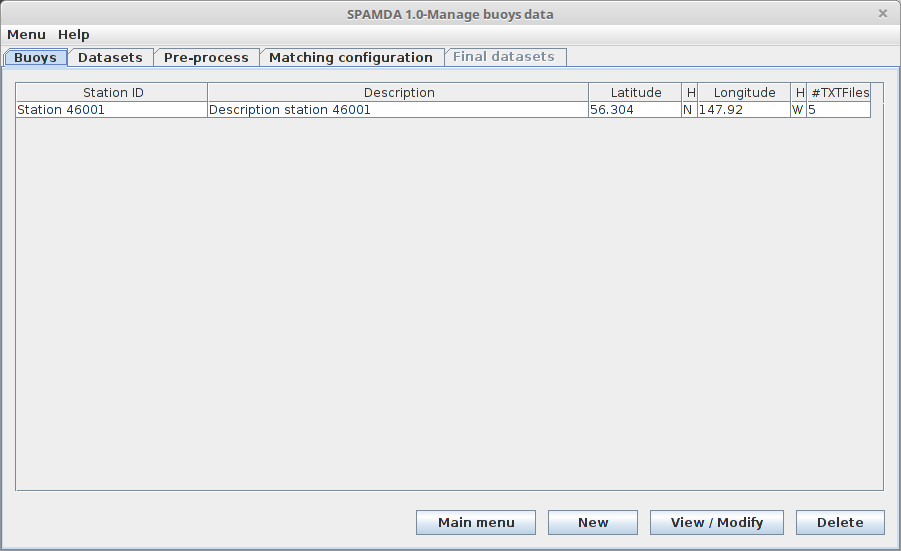
\includegraphics[width=0.89\textwidth]{figures/FigureManage_buoys.png}
				\caption{\textit{Buoys} tab: buoy ID 46001.}\label{fig:manage_buoys}
			\end{figure}
			
			After that, the researcher has to select \textbf{\textit{Manage buoys data}} to open the view shown in Fig. \ref{fig:manage_buoys}, where several tabs are available. In \textbf{\textit{Buoys}} tab, the researcher can consult, modify, add or delete different data related to the buoy.
			
			In order to enter such data, click on the \textbf{\textit{New}} button, and then the view shown in Fig. \ref{fig:new_buoy} pops up.

			\begin{figure}[ht!]
				\centering
				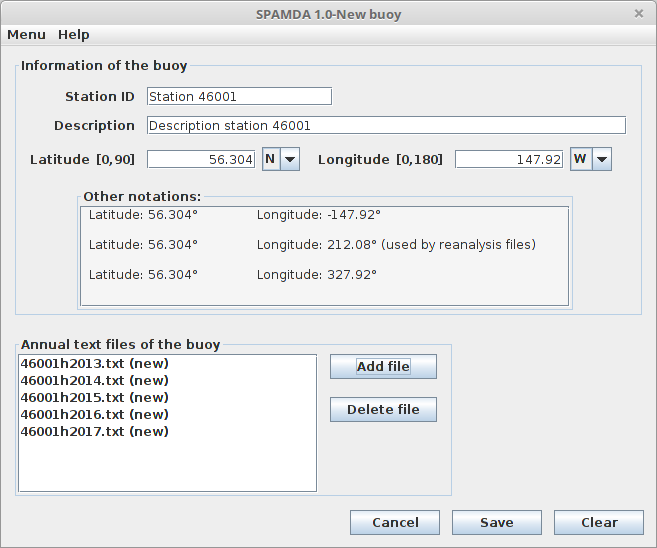
\includegraphics[width=0.65\textwidth]{figures/FigureNew_buoy.png}
				\caption{\textit{New buoy} view: information of the buoy ID 46001.}\label{fig:new_buoy}
			\end{figure}
			
			Here the information about the buoy has to be included: the \textit{Station ID}, its description, geographical localisation and the corresponding annual text files. In this case, the files containing the data from year $2013$ to $2017$ are inserted by clicking on the \textbf{\textit{Add file}} button. Once the data has been introduced, it is necessary to click on the \textbf{\textit{Save}} button to insert the buoy in SPAMDA database. After that, the view can be closed.  
		
			\begin{figure}[ht!]
				\centering
				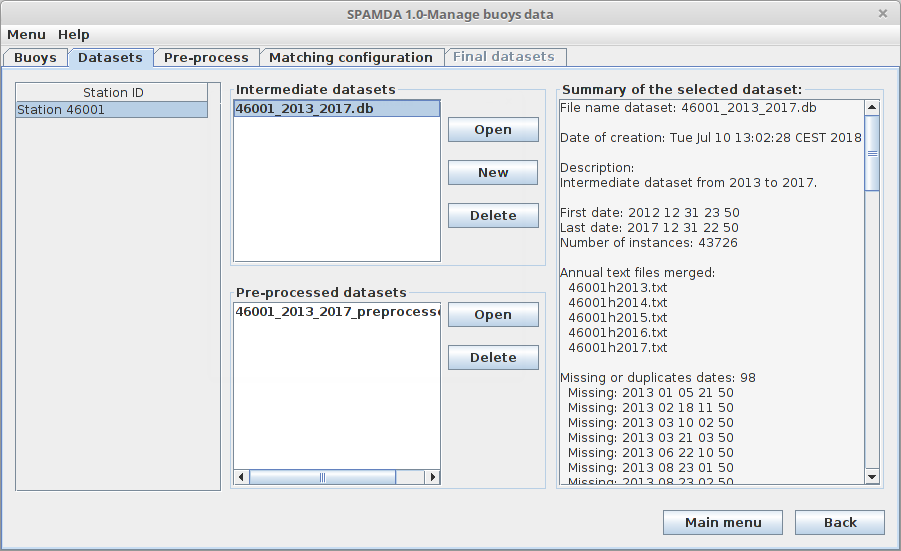
\includegraphics[width=0.83\textwidth]{figures/FigureDatasets.png}
				\caption{\textit{Datasets} tab: intermediate datasets of the buoy ID 46001.}\label{fig:show_datasets}
			\end{figure}
			
			To create the intermediate dataset, the researcher has to double-click on the buoy under study or click on the \textbf{\textit{Datasets}} tab (see Fig. \ref{fig:manage_buoys}) to switch to the corresponding view (see Fig. \ref{fig:show_datasets}). In this view, the researcher can delete or consult a summary of each intermediate or pre-processed dataset by selecting it from the corresponding list. It can also create new ones. To proceed with the creation of the intermediate dataset, the user clicks on the \textbf{\textit{New}} button, and the view shown in Fig. \ref{fig:intermediate} appears. 
			
			\begin{figure}[ht!]
				\centering
				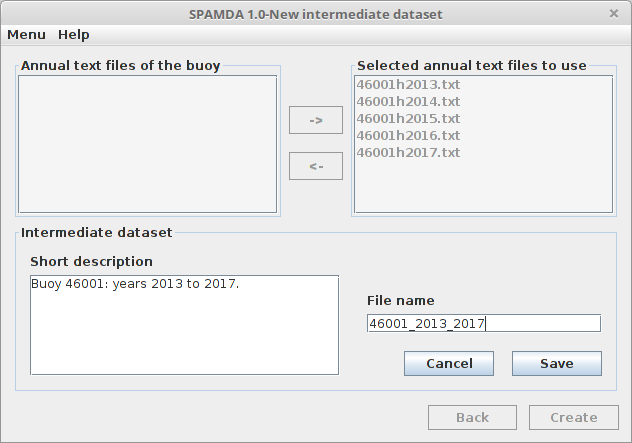
\includegraphics[width=0.67\textwidth]{figures/FigureNew_intermediate_dataset.png}
				\caption{\textit{New intermediate dataset} view: creating the intermediate dataset with $5$ annual text files.}\label{fig:intermediate}
			\end{figure}
			
			Here the researcher can select the annual text files to be included in the intermediate dataset, by clicking on the \textbf{\textit{->}} and \textbf{\textit{<-}} buttons. In this case, all the files introduced before, which correspond to the buoy under study, are selected. When the file selection is finished, \textbf{\textit{Create}} button has to be clicked in order to introduce the description and the file name of the current intermediate dataset, and then, with the \textbf{\textit{Save}} button, the creation process starts, showing the status of the process during it. After that, in order to prepare the intermediate dataset, the dataset is selected (see Fig. \ref{fig:show_datasets}), and then the button \textbf{\textit{Open}} is clicked to jump to the tab \textbf{\textit{Pre-process}} (shown in Fig. \ref{fig:preprocess_data}).
			
			\begin{figure}[ht!]
				\centering
				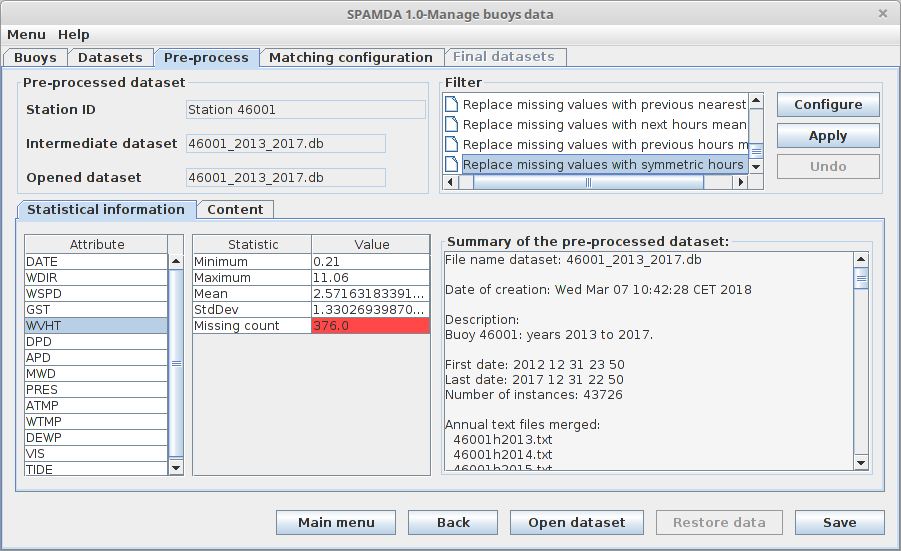
\includegraphics[width=0.84\textwidth]{figures/FigurePreprocess.png}
				\caption{\textit{Pre-process} tab: pre-processing the created intermediate dataset.}\label{fig:preprocess_data}
			\end{figure}
			
			In \textbf{\textit{Pre-process}} tab, relevant statistical information about the selected dataset is shown, and also the content of the dataset can be consulted, providing the researcher the capacity to evaluate the pre-processing being performed. Here the researcher can apply (and configure) the necessary filters (explained in Section \ref{sec:Preprocess}) to the selected dataset, and, in the bottom part, the main statistics of the dataset are displayed, which can be used to observe the changes produced when applying a filter. As mentioned earlier, this case study is focused on classifying waves considering their height, so any missing data from wave height ($376$ values) and the remaining attributes are recovered, using the filter \textit{Replace missing values with symmetric $3$ hours mean}. Furthermore, the attributes MWD, DEWP, VIS and TIDE are removed from the dataset by applying the filter \textit{RemoveByName}, since the first two had more than $92$\% of missing data and the last two $100$\%. After finishing the pre-processing of the dataset, the researcher can click on the \textbf{\textit{Save}} button, to introduce the description and file name for the current pre-processed dataset.
			
			At this point, the researcher has registered the buoy in SPAMDA, then entered its raw data and selected the required data for the problem (intermediate dataset). Finally, the data has been pre-processed in order to be ready for its future use in ML algorithms. Then, a data integration process can be carried out to merge the processed data from NDBC with the reanalysis data (also included previously) from NNRP.
			
			\begin{figure}[ht!]
				\centering
				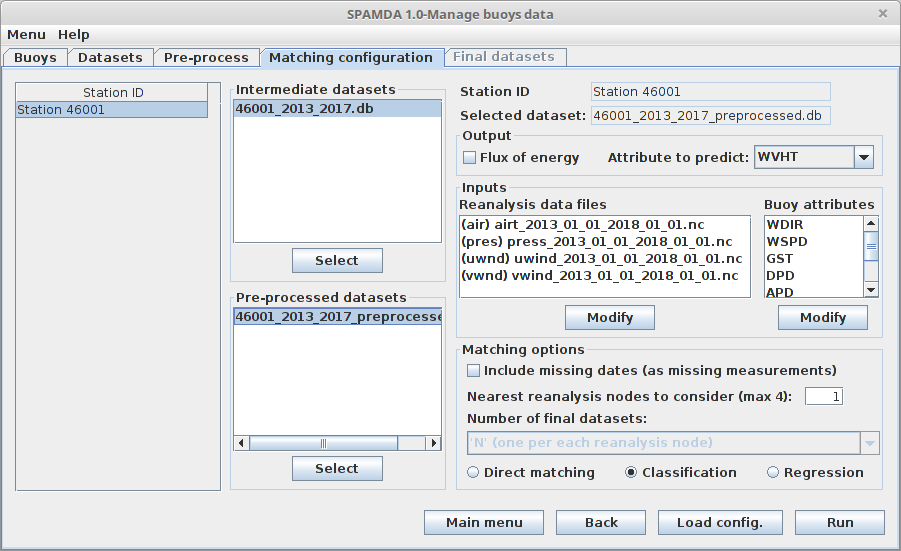
\includegraphics[width=0.84\textwidth]{figures/FigureMatching_configuration.png}
				\caption{\textit{Matching configuration} tab: parameters for the data integration of the intermediate dataset and the reanalysis files (waves classification).}\label{fig:matching_conf_wc}
			\end{figure}
			
			The next step is to customise (or load) the parameters of the matching process according to the problem being studied and to select the prediction task (described in Section \ref{sec:matching_conf}) that the final dataset will be used for, in this case, waves classification or energy flux prediction.
			
			\subsection{Waves classification}
			
			As mentioned above, the objective of the final dataset is to be used with SC and ML algorithms to classify waves depending on their significant height. Following sections describe the procedure of performing the data integration provided by SPAMDA, modelling wave height by using classification algorithms available in WEKA.
			
			\subsubsection{Obtaining the final dataset}
			
			By clicking on the \textbf{\textit{Matching configuration}} tab, the view shown in Fig. \ref{fig:matching_conf_wc} will be opened. In this view, the researcher can configure the parameters of the data integration process. For this problem, the following parameters were selected:
			
			\begin{itemize}
				\item Attribute to predict: WVHT.
				\item Reanalysis data: Air, pressure, u-wind and v-wind.
				\item Buoy attributes to be used as inputs: WDIR, WSPD, GST, DPD, APD, PRES, ATMP and WTMP (see Table \ref{tab:measurementsDescription} or descriptions of the measurements in the NDBC website).
				\item Reanalysis nodes to consider: $1$ (only the closest reanalysis node will be used).
				\item Number of final datasets: In this example that option is disabled, because only one reanalysis node is considered.
				\item Prediction task: Classification.
			\end{itemize} 
			
			\begin{figure}[ht!]
				\centering
				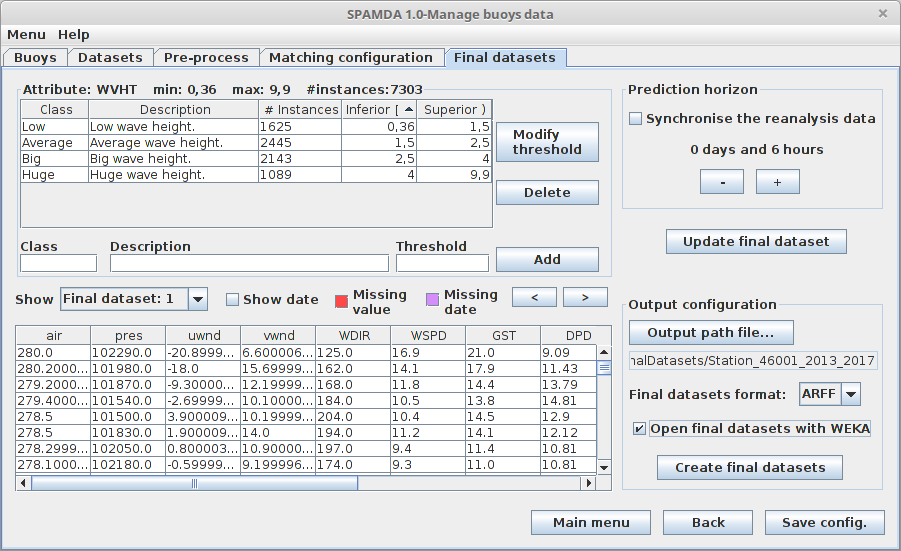
\includegraphics[width=0.90\textwidth]{figures/FigureFinal_datasets.png}
				\caption{\textit{Final datasets} tab: content of the final dataset created after data integration and discretisation of the output variable in $4$ classes.}\label{fig:final_dataset}
			\end{figure}
			
			After configuring the matching process, the researcher can click on the \textbf{\textit{Run}} button to jump to the view shown in Fig. \ref{fig:final_dataset} and proceed to define the final dataset structure according to the selected prediction task. Given that, in the previous view (Fig. \ref{fig:matching_conf_wc}), \textit{Classification} was selected, the researcher can now add, modify or delete the thresholds (usually defined by an expert) for discretising the output variable (top left of Fig. \ref{fig:final_dataset}). After this, the next step is to set the time horizon desired (6 hours by default) and also to activate (if desired) the synchronisation (in time) of reanalysis variables with the output (top right of Fig. \ref{fig:final_dataset}), as explained in Section {\ref{sec:FinalDatasets}}. Then the researcher can click on the \textbf{\textit{Update final dataset}} button to see the content shown in the bottom left corner (NDBC observations, NNRP variables, missing values, dates). Finally, after checking that everything is correct, the last step would be to select the name and path of the dataset file, and its output format (CSV or ARFF) and click on the \textbf{\textit{Create final datasets}} button (bottom right of Fig. \ref{fig:final_dataset}). For this example, the following configuration was applied:
			\begin{itemize}
				\item Thresholds: see Table \ref{tab:thresholds}.
				\item Prediction horizon: 6 hours.
				\item Synchronisation: Disabled.
				\item Final dataset format: ARFF.
			\end{itemize}
			
			At this point, the final dataset would be created according to the tailored configuration and stored in the computer of the researcher, which already can apply the ML techniques to address the problem of wave classification. Concretely, the final dataset consists of $7302$ instances and whose distribution is represented in Table \ref{tab:datasetDistribution}.
			%
				\begin{table}[!h]%
					\caption{Distribution of instances of the final dataset}
					\label{tab:datasetDistribution}
					\centering
					\begin{tabular}{cc}
						\cline{1-2}
						\textbf{Year}&\textbf{Number of instances}\\
						\cline{1-2}
						$2013$&$1460$\\
						$2014$&$1460$\\
						$2015$&$1460$\\
						$2016$&$1464$\\
						$2017$&$1458$\\
						\cline{1-2}
						&$7302$\\
						\cline{1-2}
					\end{tabular}
				\end{table}
		%
		\subsubsection{Obtaining classification models with ML algorithms}
		
			Now, the process to obtain wave classification models is described using the final dataset previously created with SPAMDA. The modelling will be performed using WEKA as SC and ML tool, which can be opened through SPAMDA, as shown in Fig. \ref{fig:openigFinalDatasetWeka}. Nevertheless, as mentioned above, the researcher can create the final dataset in CSV format in order to use any other ML tools, such as KEEL, Python or R, among others.
			
			\begin{figure}[ht!]
				\centering
				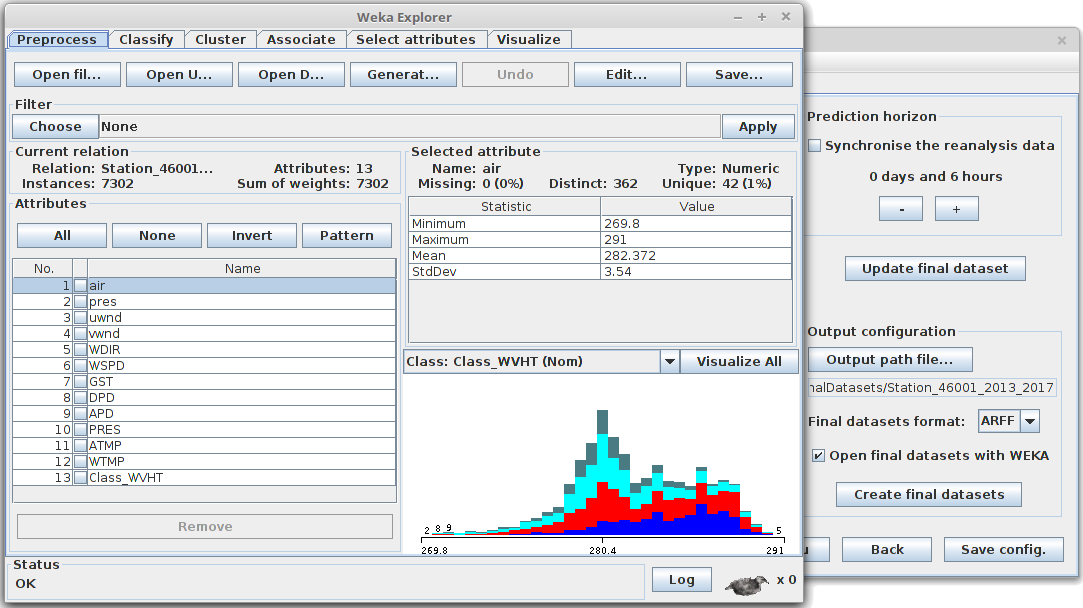
\includegraphics[width=0.95\textwidth]{figures/FigureOpeningFinalDatasetWeka.png}
				\caption{Final dataset opened with the environment Explorer of WEKA (waves classification).}
				\label{fig:openigFinalDatasetWeka}
			\end{figure}
			
			Since the final dataset is a time series of meteorological data (collected from $2013$ to $2017$), a hold-out scheme (60\% train / 40\% test) will be used. In this way, years from $2013$ to $2015$ will be used for the training phase ($4380$ instances) whereas $2016$ and $2017$ years will be used for the test phase ($2922$ instances). Previous to the learning phase, the attributes are normalised to avoid that some attributes dominate others because of a larger scale.
			
			The classification algorithms that will be considered for wave modelling are Logistic Regression \cite{hosmer2013applied}, C4.5 \cite{quinlan2014c4}, Random Forest \cite{breiman2001random}, Support Vector Machine \cite{cortes1995support} and Multilayer Perceptron \cite{haykin1994neural}, which will be applied with the default values of the parameters provided by WEKA. Given that Logistic Regression and C4.5 algorithms are deterministic, only one run will be considered for each one. However, Random Forest, Support Vector Machine and Multilayer Perceptron algorithms have a stochastic component, so, in this case, 30 executions for each one will be carried out. Table \ref{tab:results} shows the results of this experimentation.
			
				\begin{table}[!h]
				
					\caption{Results (mean$\pm$SD) obtained by the algorithms}
					\label{tab:results}
					\footnotesize
					\centering

					\begin{tabular}{m{3.20cm}cc@{\setlength{\tabcolsep}{0pt}}m{0.0cm}}
					
						\cline{1-4}
						
						\textbf{Algorithm}&\textbf{Accuracy (CCR)}&\textbf{Kappa}&\\[0.20cm]
	
						\cline{1-4}
						
						Logistic Regression & $59.0691$ & $0.44447$&\\[0.15cm]
						
						\cellcolor{gray090}C4.5 & \cellcolor{gray090}$61.7385$ & \cellcolor{gray090}$0.47852$&\\[0.15cm]
						
						Random Forest & $\textit{68.6516} \pm \textit{0.3083}$ & $\textit{0.57040} \pm \textit{0.0042}$&\\[0.15cm]
						
						\cellcolor{gray090}Support Vector Machine &\cellcolor{gray090} $61.0016 \pm 0.0522$ &\cellcolor{gray090} $0.46770 \pm 0.0007$&\\[0.15cm]
						
						Multilayer Perceptron & $\mathbf{69.7045} \pm \mathbf{1.3033}$ & $\mathbf{0.58576} \pm \mathbf{0.0178}$&\\[0.15cm]

						\cline{1-4}
							
					\end{tabular}
				
				\end{table}
				
			As can be seen, Random Forest and Multilayer Perceptron algorithms have achieved similar accuracy, but the performance of the latter is slightly better. Although this is an illustrative classification example using datasets built with SPAMDA, both models have obtained good performance, despite the problem tackled is difficult (prediction is approached six hours in advance).
			
			\subsection{Energy flux prediction}
			
			As mentioned above, the final dataset of this example is also used with SC and ML algorithms to predict flux of energy. Following sections explain the process of performing the data integration provided by SPAMDA to build the final dataset, modelling the flux of energy by using regression algorithms available in WEKA.
			
			\subsubsection{Obtaining the final dataset}
			
			The researcher can configure the parameters of the data integration by clicking on the \textbf{\textit{Matching configuration}} tab. For this problem, as shown in Fig. \ref{fig:matching_conf_ef}, the following parameters were selected:

			\begin{itemize}
				\item Attribute to predict: Flux of energy.
				\item Reanalysis data: Air, pressure, u-wind and v-wind.
				\item Buoy attributes to be used as inputs: WDIR, WSPD, GST, DPD, APD, PRES, ATMP and WTMP (see Table \ref{tab:measurementsDescription} or descriptions of the measurements in the NDBC website).
				\item Reanalysis nodes to consider: $1$ (only the closest reanalysis node will be used).
				\item Number of final datasets: In this example, this option is disabled, because only one reanalysis node is considered.
				\item Prediction task: Regression.
			\end{itemize} 
			
			\begin{figure}[ht!]
				\centering
				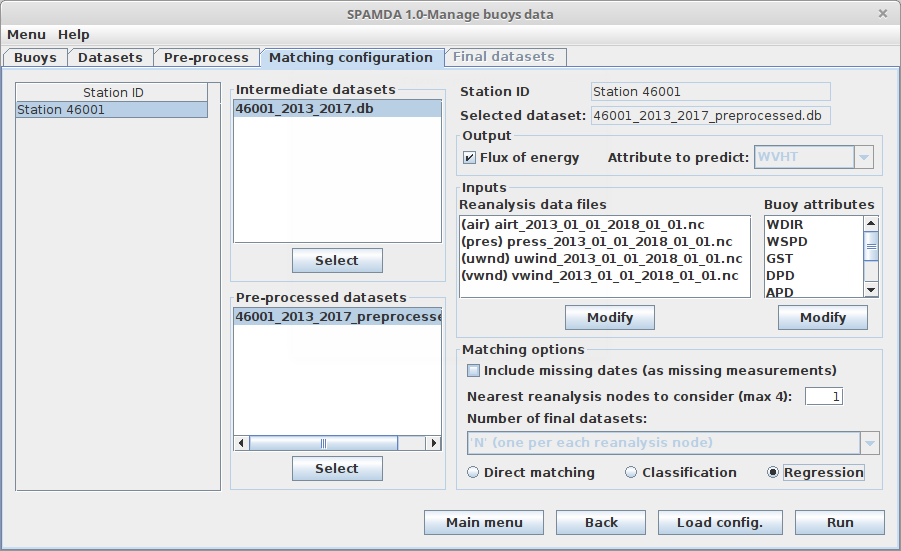
\includegraphics[width=0.85\textwidth]{figures/FigureMatching_configuration_EF.png}
				\caption{\textit{Matching configuration} tab: parameters for the data integration of the intermediate dataset and the reanalysis files (energy flux prediction).}\label{fig:matching_conf_ef}
			\end{figure}

			\begin{figure}[ht!]
				\centering
				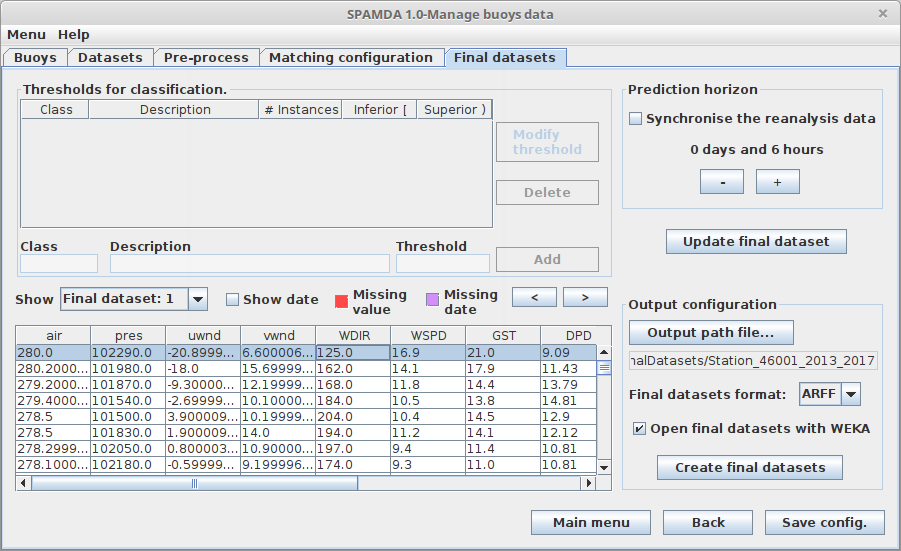
\includegraphics[width=0.85\textwidth]{figures/FigureFinal_datasets_EF.png}
				\caption{\textit{Final datasets} tab: content of the final dataset created after data integration.}\label{fig:final_dataset_EF}
			\end{figure}
			
			After configuring the parameters of the matching process, the next step is to define the final dataset structure according to the selected prediction task. Researcher can click on the \textbf{\textit{Run}} button to jump to the view shown in Fig. \ref{fig:final_dataset_EF}. Note that, the thresholds for discretising the output variable (top left of Fig. \ref{fig:final_dataset_EF}) are disabled due to, in this case, energy flux prediction is a regression problem.

			By default, the time horizon is set to $6$ hours, that is, the energy flux prediction will be performed $6$ hours in advance (top right of Fig. \ref{fig:final_dataset_EF}), but researchers can increase such time horizon depending on their needs. The synchronisation (in time) of reanalysis variables with the output (explained in Section {\ref{sec:FinalDatasets}}) can be set in this view. By clicking on the \textbf{\textit{Update final dataset}} button, researchers can preview the content of the final dataset (bottom left corner of Fig. \ref{fig:final_dataset_EF}). Finally, the last step would be to set the name, path and output format (CSV or ARFF) of the dataset file, and then the user should click on the \textbf{\textit{Create final datasets}} button (bottom right of Fig. \ref{fig:final_dataset_EF}). For this example, the following configuration was applied:

			\begin{itemize}
				\item Prediction horizon: 6 hours.
				\item Synchronisation: Disabled.
				\item Final dataset format: ARFF.
			\end{itemize}
			
			After that, the final dataset would be created and stored in the computer of the researcher according to the introduced configuration, ready to be used as input for SC and ML techniques to tackle the problem of energy flux prediction. The number of instances ($7302$) and the distribution of the final dataset (Table \ref{tab:datasetDistribution}) are the same as in the previous example (waves classification) since the data used to create the final dataset and the time horizon selected (6h) are the same.

		\subsubsection{Obtaining prediction models with ML algorithms}

			In this example, WEKA is used as SC and ML tool to obtain energy flux prediction models, as shown in Fig. \ref{fig:openigFinalDatasetWeka_EF}. Nonetheless, the final dataset can be created in CSV format so that the researcher can use any other SC and ML tool.

			\begin{figure}[ht!]
				\centering
				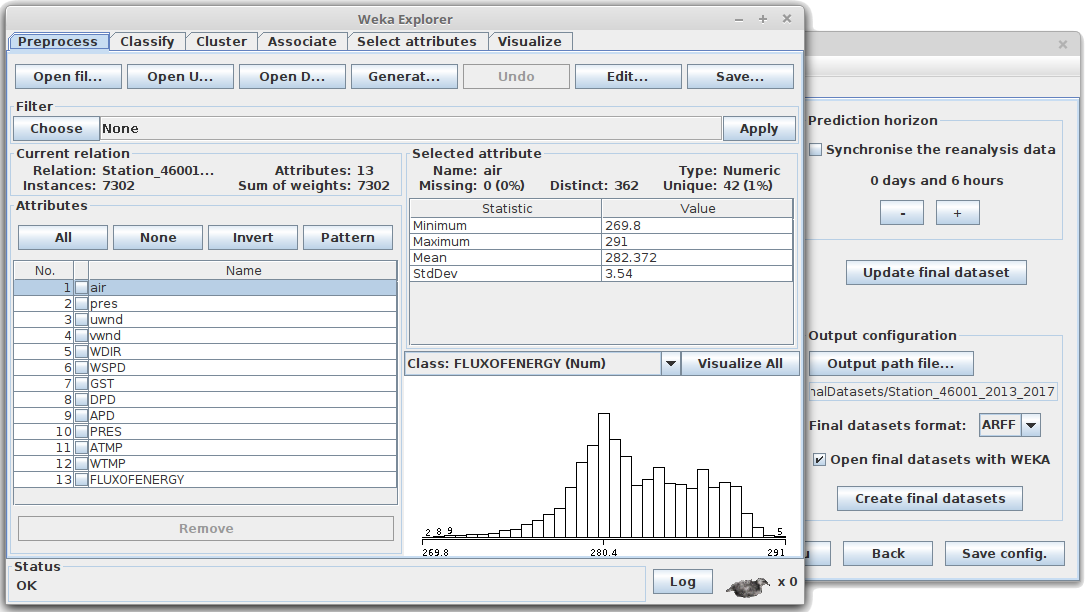
\includegraphics[width=0.95\textwidth]{figures/FigureOpeningFinalDatasetWeka_EF.png}
				\caption{Final dataset opened with the environment Explorer of WEKA (energy flux prediction).}
				\label{fig:openigFinalDatasetWeka_EF}
			\end{figure}
			
			For this problem, the same partitioning scheme used in the wave classification problem is considered (60\% train / 40\% test), that is, years from $2013$ to $2015$ for the training phase ($4380$ instances) and years $2016$ and $2017$ for the test phase ($2922$ instances). Again, the attributes are normalised prior to the learning phase.
			
			To perform the energy flux modelling, one execution will be run for the deterministic algorithm Linear Regression \cite{Bishop:2006:PRM:1162264}, whereas $30$ executions will be considered for the stochastic ones: Random Forest \cite{breiman2001random}, Support Vector Machine \cite{cortes1995support} and Multilayer Perceptron \cite{haykin1994neural}. Table \ref{tab:results_EF} shows the experimental results obtained using the default values for the parameters of the algorithms provided by WEKA.

				\begin{table}[!h]
				
					\caption{Results (mean$\pm$SD) obtained by the algorithms}
					\label{tab:results_EF}
					\footnotesize
					\centering

					\begin{tabular}{m{3.20cm}cc@{\setlength{\tabcolsep}{0pt}}m{0.0cm}}
					
						\cline{1-4}
						
						\textbf{Algorithm}&\textbf{Root mean squared error}&\textbf{Correlation coefficient}&\\[0.20cm]
	
						\cline{1-4}
						
						Linear Regression & $29.6368$ & $0.7296$&\\[0.15cm]
						
						\cellcolor{gray090}Random Forest &\cellcolor{gray090} $\mathbf{23.4353} \pm \mathbf{0.1313}$ &\cellcolor{gray090} $\textit{0.8408} \pm \textit{0.0021}$&\\[0.15cm]
						
						Support Vector Machine & $31.3008 \pm 0.1197$ & $0.7275 \pm 0.0015$&\\[0.15cm]
						
						\cellcolor{gray090}Multilayer Perceptron &\cellcolor{gray090} $\textit{27.1151} \pm \textit{7.5536}$ &\cellcolor{gray090} $\mathbf{0.8444} \pm \mathbf{0.0193}$&\\[0.15cm]

						\cline{1-4}
							
					\end{tabular}
				
				\end{table}
			
			As can be checked, Random Forest has achieved the best performance for the Root mean squared error. The standard deviation of the results obtained by Multilayer Perceptron indicates that this algorithm may has been slightly affected by its stochastic component. However, both Multilayer Perceptron and Random Forest have obtained an excellent Correlation coefficient.
			
			In this case study, the use of datasets created with SPAMDA has been shown to address an energy flux prediction problem. An exhaustive comparison of regression algorithms is not the purpose of this work. However, note that Multilayer Perceptron and Random Forest algorithms have achieved very good results despite the fact that the energy flux prediction has been performed with a time horizon of 6h.

		\subsection{Important remarks}
		
			In this section, it has been described how to use SPAMDA to create final datasets with the aim of classifying waves and predicting flux of energy. However, using the same data described in Section \ref{sec:ObtainingFinalDataset} the researcher can quickly address other objectives or different studies by merely tailoring the matching configuration of the data integration process. For example, longer-term wave or energy flux prediction can be addressed by changing the time horizon, waves modelling can be approached from another perspective by creating the final dataset for regression, or environmental modelling can be focused in diverse fields by changing the output meteorological variable.

			Furthermore, environmental modelling in other geographical location can be carried out by merely using other collected data.
			
			As SPAMDA performs all data processing and management to create the datasets, it not only prevents researchers from performing repetitive tasks but also prevents them from making possible errors. In this way, researchers can focus on the studies they are carrying out.
		
	\section{Conclusions}\label{sec:Conclusions}

		%A new open source tool named SPAMDA with an user-friendly GUI for creating datasets using meteorological data from NDBC and NNRP has been presented in this work. The aim of the tool presented in this work is to provide the research community with an automated, customisable and robust integration for NDBC and NNRP data, serving as a tool for analysis and decision support in marine energy and engineering applications, among others.
		
		%Studies on marine energy using ML and SC methodologies apply specific algorithms (extreme learning machine, metaheuristics, Bayesian networks, neural networks, etc) on data using custom-made implementations or scripts developed in some programming language; but they do not allow to build datasets in an automated way ready to be used as input for prediction tasks (classification or regression). These datasets can be easily obtained with SPAMDA by means of the selection of different input parameters, such as predictive and objective variables, output discretisation or prediction horizon. As a result, researchers will benefit from significant support when carrying out environmental modelling related to energy, atmospheric or oceanic studies, among others. Moreover, given that SPAMDA simplifies all the intermediate steps involved in the creation of datasets and manages the extensive casuistry of the data integration (such as entering the meteorological information, managing with the incomplete data, pre-processing tasks, the customisable matching process to merge the data and the preparation of the datasets according to the SC or ML technique to use), it avoids errors and reduces the time needed. In this way, researchers will be able to have more in-depth analysis, which could result in more complete conclusions about the issue under study.
		
		\textcolor{blue}{Studies on marine energy using ML and SC methodologies apply specific algorithms (extreme learning machine, metaheuristics, Bayesian networks, neural networks, etc.) on data using custom-made implementations or scripts developed in some programming language; but they do not allow to build datasets in an automated way ready to be used as input for prediction tasks (classification or regression). In this sense, a new open source tool named SPAMDA has been presented in this work, with an user-friendly GUI for creating datasets using meteorological data from NDBC and NNRP. The aim of the tool is to provide the research community with an automated, customisable and robust integration for NDBC and NNRP data, serving as a tool for analysis and decision support in marine energy and engineering applications, among others.}
		
		Such datasets can be easily obtained with SPAMDA by means of the selection of different input parameters, such as predictive and objective variables, output discretisation or prediction horizon. As a result, researchers will benefit from significant support when carrying out environmental modelling related to energy, atmospheric or oceanic studies, among others. Moreover, given that SPAMDA simplifies all the intermediate steps involved in the creation of datasets and manages the extensive casuistry of the data integration (such as specifying the meteorological information, managing incomplete data, pre-processing tasks, the customisable matching process to merge the data and the preparation of the datasets according to the SC or ML technique to use), it avoids errors and reduces the time needed. In this way, researchers will be able to have more in-depth analysis, which could result in more complete conclusions about the issue under study.
		
		The case study described in Section \ref{sec:CaseStudy} illustrates how SPAMDA can be used by researchers in a practical approach for environmental modelling, concretely, to classify waves in the Gulf of Alaska depending on their height. The case study also covers an example of energy flux prediction, to predict the wave energy that could be exploited by WECs facilities six hours in advance, although such time horizon is customisable. Given that this work does not focus on models performance, a more extensive validation or comparison study of the results obtained in both examples has not been carried out. \textcolor{blue}{The final datasets obtained with SPAMDA can be replicated by researchers using the same meteorological data from NDBC and NNRP (publicly available) and applying the same parameters for the pre-processing tasks and the data integration process. After that, the models and results obtained, using such final datasets, will depend on the SC or ML tool used.}

		In order to improve SPAMDA, some future work could be focused on new functional modules for managing meteorological data of different formats \cite{NOAA_3}, so that the developed tool can be extended to any other research, new pre-processing functionalities such as filters to analyse the correlation between attributes or new functional modules for recovering missing values using nearby buoys data \cite{DuranRosal2016}. Furthermore, the developed software could manage other sources of reanalysis data (with different spatial and temporal resolution), and new output formats for the datasets which could be used as input by other tools for ML such as KEEL (\textit{Knowledge Extraction based on Evolutionary Learning}) \cite{AlcalFdez2009KEELAS}. However, such new functionalities can be developed with a reasonable effort to be able to manage each particular casuistry. For example, when dealing with incomplete data, interpreting different data and files structures or carrying out the matching process of two environmental data sources.

    \section*{Additional material}
	
		The source code and the software tool are available at \url{https://github.com/ayrna}.

%%%%%%%%%%%%%%%%%%%%%%%%%%%%%%%%%%%%%%%%%%
\vspace{6pt} 

%%%%%%%%%%%%%%%%%%%%%%%%%%%%%%%%%%%%%%%%%%
%% optional
%\supplementary{The following are available online at \linksupplementary{s1}, Figure S1: title, Table S1: title, Video S1: title.}

% Only for the journal Methods and Protocols:
% If you wish to submit a video article, please do so with any other supplementary material.
% \supplementary{The following are available at \linksupplementary{s1}, Figure S1: title, Table S1: title, Video S1: title. A supporting video article is available at doi: link.}

%%%%%%%%%%%%%%%%%%%%%%%%%%%%%%%%%%%%%%%%%%
%\authorcontributions{For research articles with several authors, a short paragraph specifying their individual contributions must be provided. The following statements should be used ``Conceptualization, X.X. and Y.Y.; methodology, X.X.; software, X.X.; validation, X.X., Y.Y. and Z.Z.; formal analysis, X.X.; investigation, X.X.; resources, X.X.; data curation, X.X.; writing--original draft preparation, X.X.; writing--review and editing, X.X.; visualization, X.X.; supervision, X.X.; project administration, X.X.; funding acquisition, Y.Y. All authors have read and agreed to the published version of the manuscript.'', please turn to the  \href{http://img.mdpi.org/data/contributor-role-instruction.pdf}{CRediT taxonomy} for the term explanation. Authorship must be limited to those who have contributed substantially to the work reported.}

\authorcontributions{Conceptualization, Formal analysis and Investigation, Antonio Manuel Gómez-Orellana, Juan Carlos Fernández, Manuel Dorado-Moreno, Pedro Antonio Gutiérrez and César Hervás-Martínez; Funding acquisition, Project administration, Resources and Supervision, Pedro Antonio Gutiérrez and César Hervás-Martínez; Methodology, Antonio Manuel Gómez-Orellana, Juan Carlos Fernández, Manuel Dorado-Moreno, Pedro Antonio Gutiérrez and César Hervás-Martínez; Software, Antonio Manuel Gómez-Orellana, Juan Carlos Fernández and Manuel Dorado-Moreno; Validation, Antonio Manuel Gómez-Orellana, Juan Carlos Fernández, Manuel Dorado-Moreno, Pedro Antonio Gutiérrez and César Hervás-Martínez; Writing – original draft, Antonio Manuel Gómez-Orellana, Juan Carlos Fernández and Manuel Dorado-Moreno.}

%%%%%%%%%%%%%%%%%%%%%%%%%%%%%%%%%%%%%%%%%%
%\funding{Please add: ``This research received no external funding'' or ``This research was funded by NAME OF FUNDER grant number XXX.'' and  and ``The APC was funded by XXX''. Check carefully that the details given are accurate and use the standard spelling of funding agency names at \url{https://search.crossref.org/funding}, any errors may affect your future funding.}

%\funding{This work has been partially subsidised by the projects with references TIN2017-85887-C2-1-P of the Spanish Ministry of Economy and Competitiveness (MI\-NE\-CO), UCO-1261651 of the ``Consejer\'ia de Econom\'ia, Conocimiento, Empresas y Universidad'' of the ``Junta de Andaluc\'ia'' (Spain) and FEDER funds of the European Union. We also thank to NVIDIA Corporation for the transfer of computational resources for research works.}

\funding{This work has been partially subsidised by the projects with references TIN2017-85887-C2-1-P of the Spanish Ministry of Economy and Competitiveness (MI\-NE\-CO), UCO-1261651 of the ``Consejer\'ia de Econom\'ia, Conocimiento, Empresas y Universidad'' of the ``Junta de Andaluc\'ia'' (Spain) and FEDER funds of the European Union.}

%%%%%%%%%%%%%%%%%%%%%%%%%%%%%%%%%%%%%%%%%%
%\acknowledgments{In this section you can acknowledge any support given which is not covered by the author contribution or funding sections. This may include administrative and technical support, or donations in kind (e.g., materials used for experiments).}

\acknowledgments{The authors also thank to NOAA/OAR/ESRL PSD, Boulder, Colorado, USA for the NCEP Reanalysis data provided from their Web site at \url{https://www.esrl.noaa.gov/psd/}, to NOAA/NDBC by its data that were collected and made freely available, to University of Waikato for the WEKA (Waikato Environment for Knowledge Analysis) software tool, to University Corporation for Atmospheric Research/Unidata for the NetCDF (network Common Data Form) Java library and to QOS.ch for the SLF4J (Simple Logging Facade for Java) library.}

%%%%%%%%%%%%%%%%%%%%%%%%%%%%%%%%%%%%%%%%%%
%\conflictsofinterest{Declare conflicts of interest or state ``The authors declare no conflict of interest.'' Authors must identify and declare any personal circumstances or interest that may be perceived as inappropriately influencing the representation or interpretation of reported research results. Any role of the funders in the design of the study; in the collection, analyses or interpretation of data; in the writing of the manuscript, or in the decision to publish the results must be declared in this section. If there is no role, please state ``The funders had no role in the design of the study; in the collection, analyses, or interpretation of data; in the writing of the manuscript, or in the decision to publish the results''.} 

%\conflictsofinterest{The authors declare no conflict of interest. The funders had no role in the design of the study; in the collection, analyses, or interpretation of data; in the writing of the manuscript, or in the decision to publish the results.} 

\conflictsofinterest{The authors declare no conflict of interest.} 

%%%%%%%%%%%%%%%%%%%%%%%%%%%%%%%%%%%%%%%%%%
%% optional
%\abbreviations{The following abbreviations are used in this manuscript:\\
\abbreviations{Abbreviations used in this manuscript:\\

% \noindent 
% \begin{tabular}{@{}ll}
% MDPI & Multidisciplinary Digital Publishing Institute\\
% DOAJ & Directory of open access journals\\
% TLA & Three letter acronym\\
% LD & linear dichroism
% \end{tabular}}

\noindent 
\begin{tabular}{@{}ll}
$F_e$ & Flux of energy\\
$H_s$ & Significant wave height\\
$T_e$ & Wave energy period\\
$p_0$ & Geographical location of the buoy\\
$p_j$ & Geographical location of each reanalysis node\\
$lat$ & Latitude of the point\\
$lon$ & Longitude of the point\\
$o_{t}$ & The attribute to be predicted at the time instant to study\\
$\Delta t$ & The prediction horizon\\
$\mathbf{b}_t$ & The vector containing the selected NDBC variables\\
$\mathbf{r}_{t}$ & The vector containing the selected reanalysis variables\\
\end{tabular}}

%%%%%%%%%%%%%%%%%%%%%%%%%%%%%%%%%%%%%%%%%%
%% optional
%\appendixtitles{no} % Leave argument "no" if all appendix headings stay EMPTY (then no dot is printed after "Appendix A"). If the appendix sections contain a heading then change the argument to "yes".
\appendixtitles{yes}

\appendix
\section{Managing the casuistry of incomplete data}\label{app:AppendixA}

		In this appendix, we describe how SPAMDA deals with incomplete data when creating intermediate datasets and performing the matching process.
		
		The measurements collected by the buoys may be incomplete or recorded at a different time than the expected one, due to the weather conditions in which the buoys have to operate. To illustrate this casuistry, the following examples are shown in Fig. \ref{fig:measurements}:		
		\begin{itemize}
			\item In the instance marked with a), the measurement of $17$:$50$ was collected at $17$:$45$, $5$ minutes earlier.
			\item In the instance marked with b), the measurement of $23$:$50$ was collected at $23$:$30$, $20$ minutes earlier.
			\item In the instance marked with c), the measurement of $05$:$50$ is duplicated.
			\item In the instance marked with d), the measurement of $11$:$50$ is missing (missing date or instance).
			\item In the instance marked with e), the measurement of $17$:$50$ and $18$:$50$ are missing (missing dates or instances).
			\item Missing values highlighted in red colour.
		\end{itemize}
		
		\begin{figure}[ht!]
			\centering
			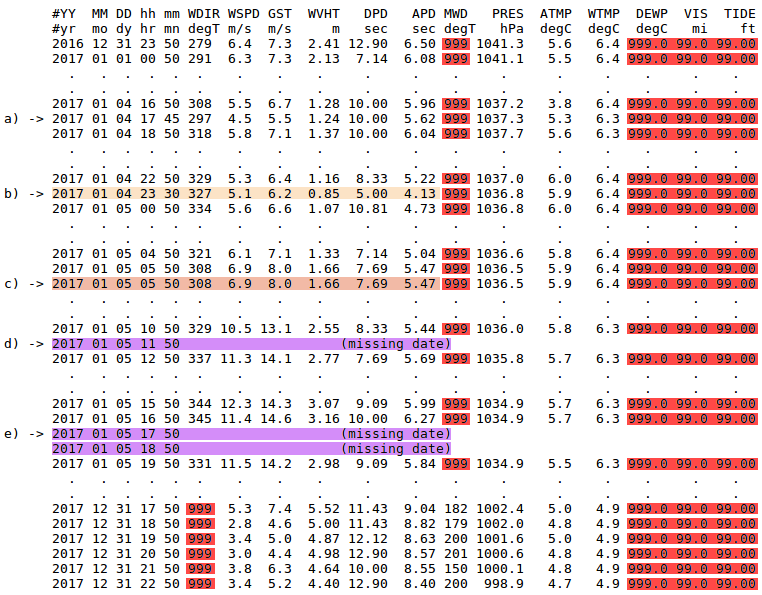
\includegraphics[scale=0.47]{figures/FigureMeasurements.png}
			\caption{A fragment of an annual text file with different missing value examples.}
			\label{fig:measurements}
		\end{figure}
		
		SPAMDA has been designed to tackle these situations, and it informs researchers of any incidence found while reading the annual text files for creating the intermediate datasets. For the case of measurements that were recorded at a different time than expected, it has been established a time gap of 6 minutes ($10\%$ of an hour). Therefore, if the time difference exceeds such value the date will be considered as an unexpected.
		
		Fig. \ref{fig:creatingDataset} shows the status of the creation of an intermediate dataset with the information of Fig \ref{fig:measurements}. Note that the instance marked with a) has not been informed by SPAMDA as an unexpected date because its time difference is less than $6$ minutes. Depending on the affected attribute, NDBC uses a specific value \cite{NOAA_3} to indicate the presence of lost data (e.g. $99$ for VIS and TIDE attributes, $999$ for DEWP, MWD and WDIR, etc.). SPAMDA interprets these specific values and, after creating the intermediate dataset, researchers can check if it contains missing values by visualising its statistical information or content. Remember that SPAMDA provides several filters for recovering missing data, which were described in subsection \ref{sec:Datasets}.
		
		\begin{figure}[ht!]
			\centering
			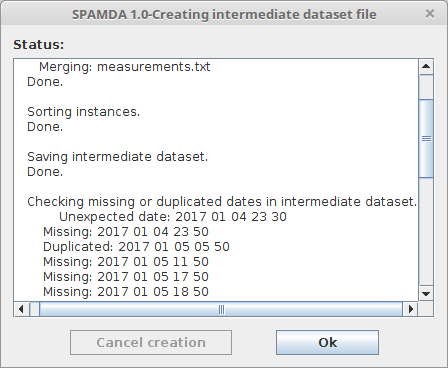
\includegraphics[scale=0.47]{figures/FigureCreatingDataset.png}
			\caption{Status of the creation of the intermediate dataset for the example of Fig \ref{fig:measurements}.}
			\label{fig:creatingDataset}
		\end{figure}
		
		SPAMDA takes into account this casuistry when carrying out the matching process. An example is given in Fig. \ref{fig:matchingMeasurements}. As above-mentioned, the matching process is performed with the nearest measurement (previous or next) within a maximum of 60 minutes of difference. However, in the instance marked with $e)$, given that the measurements dates $01$/$05$/$2017$ $17$:$50$ and $01$/$05$/$2017$ $18$:$50$ are missing, the reanalysis date $01$/$05$/$2017$ $18$:$00$ cannot be matched with buoy data (this date is highlighted in mauve colour in the Figure). Depending on the selection made by researchers in the parameter \textit{Include missing dates}, this instance will be included in the final dataset (with missing values for buoy variables) or not.
		
		\begin{figure}[ht!]
			\centering
			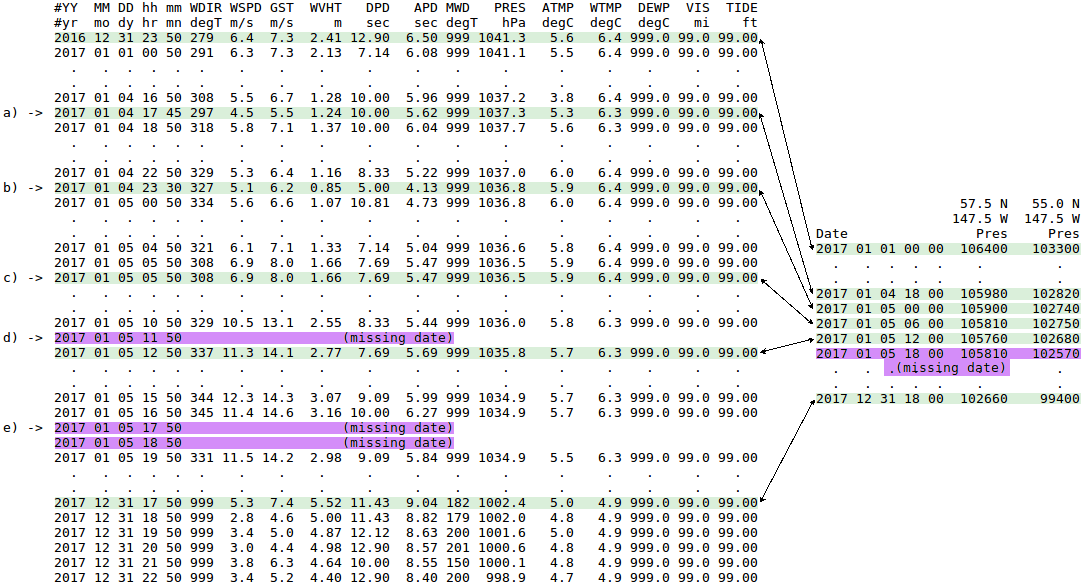
\includegraphics[scale=0.4]{figures/FigureMatchingMeasurements.png}
			\caption{Matching the measurements (left) and the reanalysis data (right).}
			\label{fig:matchingMeasurements}
		\end{figure}
		
%%%%%%%%%%%%%%%%%%%%%%%%%%%%%%%%%%%%%%%%%%
\reftitle{References}

% Please provide either the correct journal abbreviation (e.g. according to the “List of Title Word Abbreviations” http://www.issn.org/services/online-services/access-to-the-ltwa/) or the full name of the journal.
% Citations and References in Supplementary files are permitted provided that they also appear in the reference list here. 

%=====================================
% References, variant A: external bibliography
%=====================================
%\externalbibliography{yes}
%\bibliography{your_external_BibTeX_file}
\externalbibliography{yes}
\bibliography{bibfile}

%=====================================
% References, variant B: internal bibliography
%=====================================
%\begin{thebibliography}{999}
% Reference 1
%\bibitem[Author1(year)]{ref-journal}
%Author1, T. The title of the cited article. {\em Journal Abbreviation} {\bf 2008}, {\em 10}, 142--149.
% Reference 2
%\bibitem[Author2(year)]{ref-book}
%Author2, L. The title of the cited contribution. In {\em The Book Title}; Editor1, F., Editor2, A., Eds.; Publishing House: City, Country, 2007; pp. 32--58.
%\end{thebibliography}

% The following MDPI journals use author-date citation: Arts, Econometrics, Economies, Genealogy, Humanities, IJFS, JRFM, Laws, Religions, Risks, Social Sciences. For those journals, please follow the formatting guidelines on http://www.mdpi.com/authors/references
% To cite two works by the same author: \citeauthor{ref-journal-1a} (\citeyear{ref-journal-1a}, \citeyear{ref-journal-1b}). This produces: Whittaker (1967, 1975)
% To cite two works by the same author with specific pages: \citeauthor{ref-journal-3a} (\citeyear{ref-journal-3a}, p. 328; \citeyear{ref-journal-3b}, p.475). This produces: Wong (1999, p. 328; 2000, p. 475)


%%%%%%%%%%%%%%%%%%%%%%%%%%%%%%%%%%%%%%%%%%
%% optional
%\sampleavailability{Samples of the compounds ...... are available from the authors.}

%% for journal Sci
%\reviewreports{\\
%Reviewer 1 comments and authors’ response\\
%Reviewer 2 comments and authors’ response\\
%Reviewer 3 comments and authors’ response
%}

%%%%%%%%%%%%%%%%%%%%%%%%%%%%%%%%%%%%%%%%%%
\end{document}

